\documentclass[12pt]{article}

\usepackage{sbc-template}
\usepackage{graphicx,url}
\usepackage{natbib}


%\usepackage[brazil]{babel}   
\usepackage[utf8]{inputenc}  

     
\sloppy

\title{Gamified Language Learning: Enhancing Learning through Streaming Services and SRS}

\author{J. Emanuel Cascone R. S.\inst{1}, Guilherme A. Avelino\inst{1} }


\address{Computer Science Department - Federal University of Piauí (UFPI)\\
  Teresina, PI -- Brazil
  \email{\{emanuelcascone,gaa\}@ufpi.com.br}
}  
\begin{document} 

\maketitle

\begin{abstract}
  The ability to learn a new language is directly related to the user's disposition and comfort for better interaction with learning platforms. This allows for the gamification of language learning, making it less exhausting. Learning a new language typically starts with writing, reading, listening, and speaking. This project aims to create a product to facilitate language learning by using a movie streaming platform with subtitles, allowing users to watch movies with the original audio and subtitles and focus on keywords or frequently repeated words for better comprehension. The project is based on the premise that to understand a text, you don't necessarily need to know the whole formation but rather just the keywords or most repeated words, allowing you to apply skimming and scanning techniques. To record these words in the user's memory, gamified forms of Spaced Repetition System (SRS) can be applied to induce the user to better adapt to each scenario in the future based on their current repertoire. Following this approach, the user will have a better experience watching movies or videos to acquire knowledge of a new language. \\
  \textbf{Key words:} language learning, gamification, streaming platforms, subtitles, SRS, skimming, scanning
z
\end{abstract} 



\section{Introduction}


Learning a new language is essential and can benefit the individual; however, it is not always easy. Often, lack of motivation and comfort can hinder the learning process. This project aims to gamify learning new languages to overcome this obstacle, making it less exhaustive and more enjoyable.

The project consists of creating an environment using modern technologies that will possibly install a browser extension and interact with streaming sites when users watch movies with subtitles. The extension will identify the most common words in the subtitles and apply Spaced Repetition System (SRS) techniques to help the user learn the new language in a gamified manner.

Also, after watching the movie, the user can access a site or the extension by himself or download the app and continue training the words from the streaming platform. The objective is to possibilitate study in each device using the user information. 

Studies demonstrate that students acquire a new language at double the speed using a similar learning mechanism called smart subtitles \cite{Kovacs13}. Thus, it is feasible to infer that approaches involving entertainment platforms can also be practical for learning, especially when utilizing subtitles from these platforms.

The methodology adopted for the development is based on research on the process of learning new languages, as well as gamification techniques. The project will be organized into stages, starting with research and developing each environment(mobile, extension, site) and integrating those to work together.

The main objective of this project is to create a solution with well-known technologies and an excellent structure to make learning new languages more effortless and more enjoyable for the user, allowing them to utilize their free time to acquire knowledge of a new language playfully and effectively.


\subsection{Motivation}
The motivation for this project arises from the need to find alternatives to make learning a new language more exciting and efficient. The conventional language learning method can be tiresome and demotivating for many students.

By creating an environment that allows interaction with streaming sites for movies, learning a new language can be done more naturally and playfully, similar to tools that translate web pages to facilitate learning or understanding of other languages already present in the market or research area \cite{ElBatanony21}.

By watching movies with audio and subtitles in the original language, the user can learn while applying gamified SRS techniques to memorize new words. The motivation for this project is to provide an efficient and attractive alternative for learning new languages.

\subsection{Problem Statement}
The traditional method of learning a new language can be exhausting and demotivating for many students. The project aims to build another way to solve this problem. The project has an extension, site, and app to make the user experience better and more comfortable.

Also, to illustrate this, we notice that the current learning method creates a massive flow of giving up; an empirical example is "only 55, or 19\% of 286 Year 11 students reported that they intended to continue studying the language after age 16. The four most frequently cited reasons for not continuing were (a) that they did not enjoy it (35 students), (b) it was difficult (25 students), (c) it was of no use for their planned career (23 students), and (d) they were not good at it (20 students)" \cite{Graham1}.


\subsection{Teoric Referencial}
In recent years, there has been a growing interest in the use of subtitled videos as a way to assist in the learning of foreign languages. However, standard subtitles are not ideal for vocabulary acquisition, as translations are non-literal and are provided only for phrases, not individual words. To overcome this problem, "Smart Subtitles" have been developed, interactive subtitles focused on vocabulary acquisition. "Smart Subtitles" includes features such as vocabulary definitions when hovering over with the mouse cursor and video navigation based on dialogue \cite{Kovacs13}. Studies have shown that students learn more than double the vocabulary with "Smart Subtitles" compared to Chinese-English dual subtitles, with similar levels of comprehension and satisfaction \cite{Kovacs14}.


Another approach to assist in the learning of foreign languages is the use of browser extensions. The browser extension "InteractiveSubtitle" \cite{ElBatanony21} is an example of this. The extension features personalized learning, translation of phrases in context on web pages, and support for over 100 languages. The goal is to utilize various hypotheses of foreign language acquisition to create a new language learning tool that is more effective.


Based on these ideas, a browser extension has been proposed that utilizes "Smart Subtitles" to train users through gamified practice before watching a subtitled movie in a language they are learning. The extension may also aim to include features such as interactive exercises to reinforce vocabulary acquisition and games to help users practice listening and reading skills. The extension will be customized to the user's level and interests, providing an interactive and engaging learning environment.

Also, to improve the user commodity, an app and a site were proposed to not necessarily use a computer to study, providing a way for the user to study on every device.


The learn b\cite{10.1145/2939672.2939850}, \cite{10.1145/3534678.3539081}

\subsection{General goals}

This project aims to develop a browser extension that allows users to learn a new language or expand their vocabulary in a gamified and interactive manner. The extension will be designed to interact with movie streaming sites, leveraging the available subtitles on these sites to aid in the teaching process.

The project is based on the premise that learning a new language more efficiently and satisfactorily is possible when gamified and interactive. Additionally, it is based on a similar methodology - smart subtitles - which has been effective in expanding vocabulary \cite{Kovacs14}.

Thus, the goal is to offer a different and efficient approach to using subtitles so that people can learn new languages and expand their vocabulary while watching their favorite movies in a relaxed and effective way.
\subsection{Specific Objectives}

The specific objectives of this project are as follows:

\begin{itemize}
\item Develop a browser environment that could be installed or accessed by users interested in learning new languages.
\item Develop a browser extension that interacts with movie streaming sites to access the subtitles of watched films.
\item Create a keyword database for each learned language and store user information, including their progression in learning.
\item Translate the keywords into the user's language to aid comprehension.
\item Apply gamified Spaced Repetition System (SRS) techniques to help users memorize keywords in their new language.
\item Allow users to choose the language they want to learn.
\item Offer statistics on user progress, including the most challenging word, the total words learned, and others to help the user understand their learning process.
\item Provide support for multiple languages, allowing users to learn a wide range of languages using AI.
\end{itemize}

\section{Development}

The project will utilize techniques used by El Batanony et al. in their article "A browser extension to facilitate language acquisition" \cite{ElBatanony21}, making the beginning of the development a case study of their article, observing the approach they used to create an extension that interacts with web pages. Additionally, the project's path will also be based on the articles by Kovács et al. \cite{Kovacs14}, which use the premise of subtitles to advocate for a more playful and immersive learning method. This demonstrates the potential of such approaches for language learning and how more playful and intelligent approaches directly influence learning new words, as exemplified in Figure-\ref{fig:my_label}.

It also takes examples of big companies like Duolingo, Memrise, Busuu, Lingoda, Drops, and especially Language Reactor, which uses a similar approach to the project but with a different focus. 

The project was created using modern technologies, including JavaScript, Typescript, HTML, CSS, Prisma, Nextjs, PostgreSQL, and Web Channels. The project will also utilize the browser's internal messaging services to integrate the extension with streaming sites. The extension works with Prime Video, but the goal is to expand to other platforms like Netflix, Disney+, and others.

The technologies were chosen based on the need to create a fast and efficient application with a good user experience and an excellent database to store user information and progression. Nextjs is a frontend and backend that has a big community and is very fast, having a good integration with Prisma, a ORM (Object-Relational Mapping) that is easy to use and has a good amount of users with PostgreSQL database. 



\begin{figure}
\centering
\caption{Learning curves for new words using two types of subtitles and smart subtitles}
\label{fig:my_label}
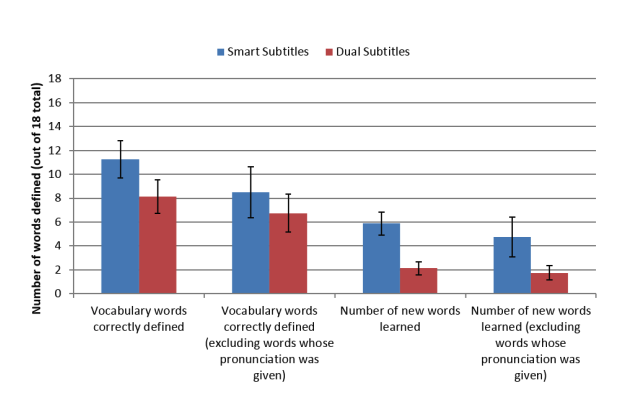
\includegraphics[width=1\textwidth]{assets/3.png}
\end{figure}

This context diagram was built to create this environment: figure-\ref{fig:context_diagram}.

\begin{figure}
\centering
\caption{
Context Diagram for the application
}
\label{fig:context_diagram}
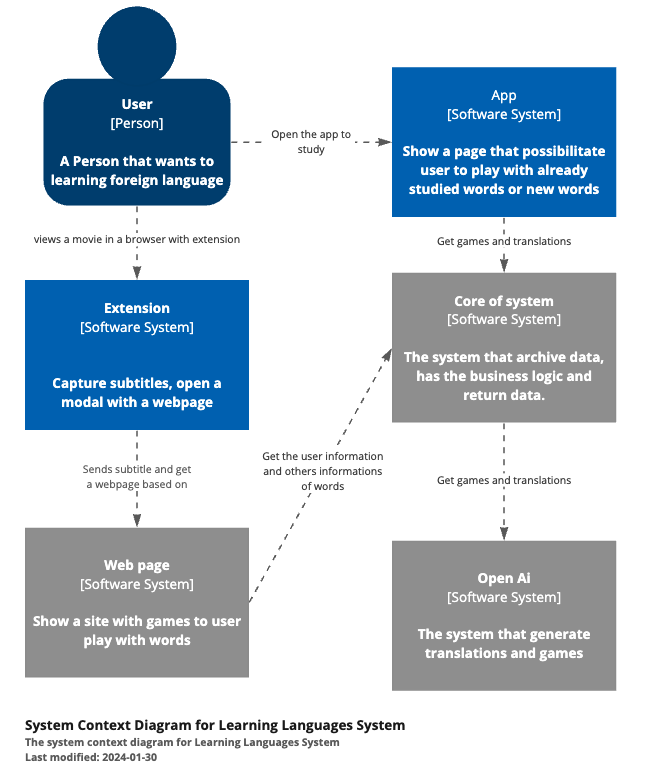
\includegraphics[width=0.5\textwidth]{assets/4.png}
\end{figure}

\subsection{Methodology}
The methodology for this project will consist of creating a browser extension that will interact with movie streaming sites and extract the subtitles available on these sites. The database stores keywords for each language and user information, including their progression in learning. The site will also provide statistics on user progress, including the most challenging words, the total words learned, and others to help the user understand their learning process, and the app will provide a way for the user to study on every device.

The extension will use Spaced Repetition System (SRS) techniques to gamify learning new languages based on the premise that knowledge of keywords or the most repeated ones allows for text comprehension.

The development of the extension was based on the following steps:
\begin{itemize}
\item Identification of streaming sites with available subtitles for movies.
\item Development of a subtitle extraction tool.
\item Integration of the extension with streaming sites.
\item Create a script to show iframe with the application site.
\item Development of teaching logic based on captured subtitles.
\item Implementation of SRS technique to gamify learning new languages.
\item Create ways to communicate between the extension, site, streaming sites, and app.
\item Integrate the extension information with the site and app.
\end{itemize}

The site: 

\begin{itemize}
\item Development of the site's graphical interface.
\item Development of the site's teaching logic based on captured subtitles.
\item Implementation of SRS technique to gamify learning new languages.
\item Create ways to communicate between the site, extension, streaming sites, and app.
\item Integrate the site information with the extension and app.
\item Create a way to update the site without user interaction.
\item Create a way to store user information, progression, keywords, and others.
\end{itemize}

The app:

\begin{itemize}
\item Development of the app's graphical interface.
\item Show the iframe with the application site.
\item Create a way to communicate between the site and the app.
\item Create a way to store site information.
\end{itemize}


And to possible future work, the project will be based on the following steps:
\begin{itemize}
\item Expansion of the extension to other streaming sites, languages, and platforms.
\item Integration of the extension with other language learning tools.
\item Development of interactive exercises and games to reinforce vocabulary acquisition.
\item Customization of the extension to the user's level and interests.
\end{itemize}

The games will display keywords during the movie playback and use SRS techniques to repeat the words spaced out, aiming to fix them in the user's memory. Additionally, the games will provide a translation of these words into the user's language to aid comprehension.

At the end of the project, it is expected to have an entire environment to learn a new language, including a browser extension, a site, and an app, all integrated and working together to provide a better experience for the user.

\begin{figure}
  \centering
  \caption{
  Database Relational Diagram for the application
  }
  \label{fig:container_diagram}
  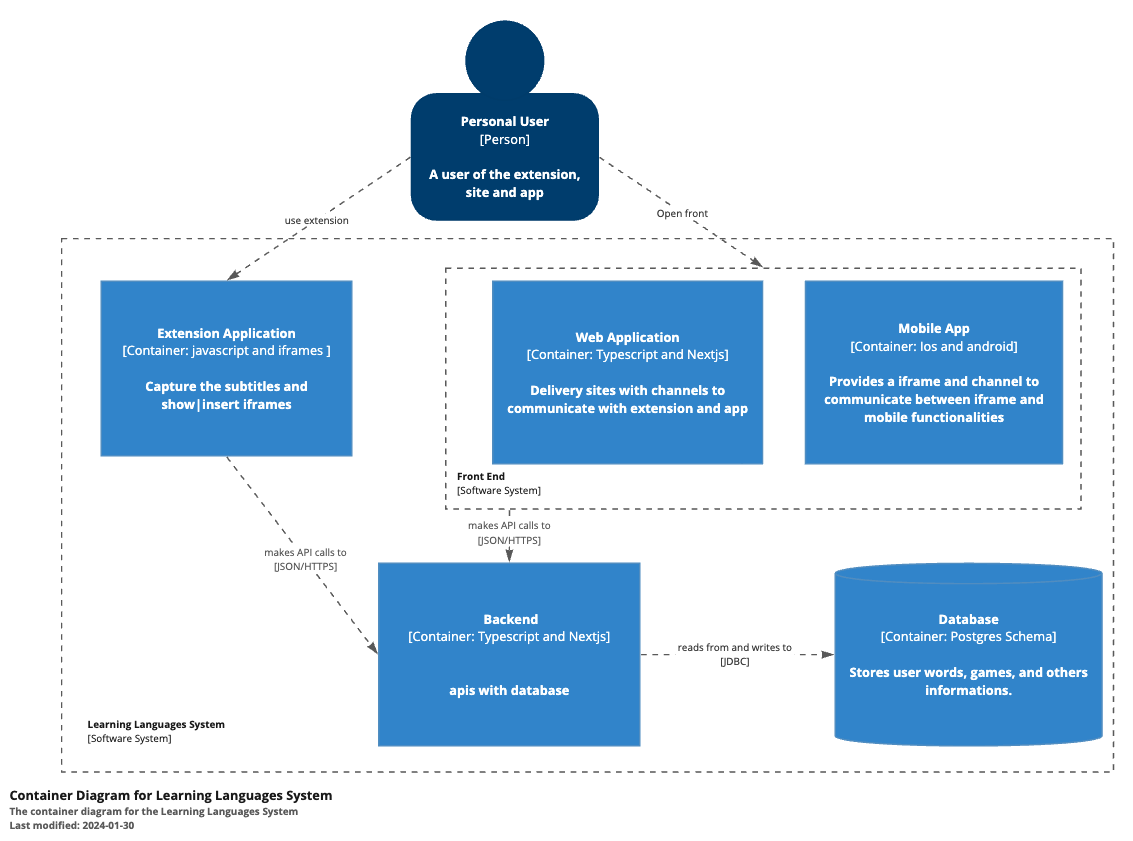
\includegraphics[width=1\textwidth]{assets/24.png}
\end{figure}



The Container diagram figure-\ref{fig:container_diagram} illustrates the project's architecture and how the extension, site, and app will interact, showing the technologies used and their communication.

\begin{figure}
  \centering
  \caption{
  Context Diagram for the application
  }
  \label{fig:database_diagram}
  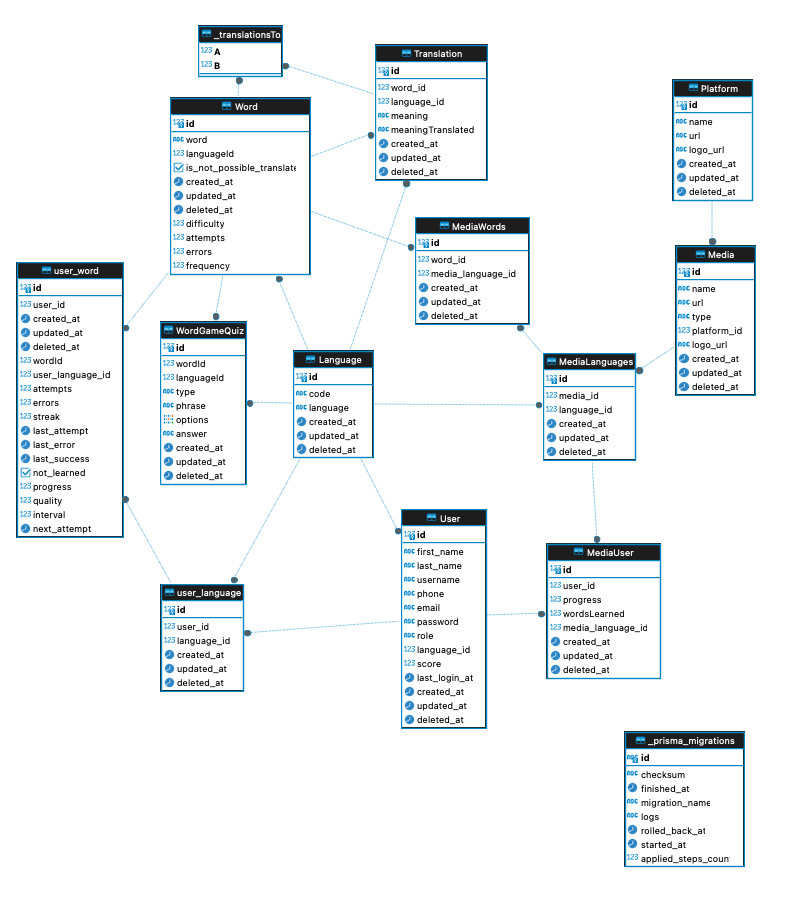
\includegraphics[width=1\textwidth]{assets/23.png}
\end{figure}


About the database structure, the diagram figure-\ref{fig:database_diagram} shows the structure of the database, including the tables and their relationships.





\subsection{Key Activities and Project Schedule}

Software implementation metrics were used to define the execution period, a backlog was created, and the development period was adapted to the time available to the student \author{J. Emanuel Cascone R. S.}.

\subsubsection{Key Activities}

The list of proposed activities is given below; each activity is transferred to the schedule detailed in Table-\ref{table:1}.

\begin{itemize}
\item Research and study of documentation on browser extensions, sites, and apps.
\item Definition of architecture and choice of technology to use.
\item Creation of the extension's graphical interface.
\item Development of subtitle capture logic.
\item Development of teaching logic based on captured subtitles.
\item Integration of subtitle capture and teaching logic.
\item Final testing of the extension.
\item Review and correction of any issues identified in final testing.
\item Preparation of technical documentation for the extension.
\item Final project delivery.
\end{itemize}


\begin{table}
\centering

\begin{tabular}{ |p{3cm}|p{3cm}|p{3cm}|p{3cm}|  }

 \hline
 \multicolumn{4}{|c|}{Schedule for project development} \\
 \hline
 \hline

\textbf{Activity} & \textbf{Description} & \textbf{Start Date} & \textbf{End Date} \\ 
\hline

Research and study & Research and study of documentation on similar platforms & 02/01/2023 & 03/01/2023 \\ \hline
Architecture definition & Definition of architecture and selection of technologies to be used & 03/02/2023 & 04/01/2023 \\ \hline
Graphical interface & Creation of the graphical interface for the platform & 04/02/2023 & 05/01/2023 \\ \hline
Subtitle capture & Development of the script for subtitle capture and processing & 05/02/2023 & 06/01/2023 \\ \hline
Data analysis & Study of possibilities for user training and important data for capture and storage & 07/01/2023 & 08/02/2023 \\ \hline
Integration & Development of the script to save and store subtitles & 09/01/2023 & 10/01/2023 \\  \hline
Testing & Testing of the created algorithms & 10/02/2023 & 11/01/2023 \\  \hline
Website, extension, and app & Integration of the created algorithms with interfaces for various environments using browser's internal messaging services & 11/02/2023 & 12/01/2023 \\ \hline
Graphic adaptation & Refactoring of the application and initiation of mini-games creation & 01/01/2024 & 02/02/2024 \\  \hline
Technical adjustments & Bug fixing and improvements & 02/03/2024 & 09/02/2024  \\
 \hline
 \end{tabular}
\caption{Table to test captions and labels.}

\label{table:1}
\end{table}

 

\subsubsection{Project Schedule and Underlying Activities}
\begin{itemize}

\item January 2023:
\begin{itemize}
\item Research and study of documentation on browser extensions, sites, and apps.
\item Study of possibilities for user training and important data for capture and storage.
\end{itemize}

\item February 2023:
\begin{itemize}
\item Start of architecture definition and choice of technology to be used.
\item Start of creation of the extension's graphical interface.
\item Conduct a literature review and gather references for similar projects or theoretical foundations.
\end{itemize}

\item March 2023:
\begin{itemize}
\item Development of logic for capturing and displaying subtitles from streaming sites.
\item Data analysis and study of possibilities for user training and important data for capture and storage.
\item Testing and improvement of subtitle capture.
\end{itemize}

\item April 2023:
\begin{itemize}
\item Development of teaching logic based on captured subtitles.
\item Integration of subtitle capture and teaching logic.
\item Testing and improvement of teaching logic.
\end{itemize}

\item August 2023:
\begin{itemize}
\item Integration of subtitle capture and teaching logic.
\item Testing and improvement of teaching logic.
\item Final testing of the extension.
\end{itemize}

\item November 2023:
\begin{itemize}
\item Review and correction of any issues identified in final testing.
\item Preparation of technical documentation for the script 
\end{itemize}

\item December 2023:
\begin{itemize}
\item Finalized script and teaching logic.
\item Start creation of the site's graphical interface.
\item Start creation of the app. 
\end{itemize}

\item January 2024:
\begin {itemize}
\item Graphic adaptation.
\item Refactoring of the application and initiation of mini-games creation.
\item Technical adjustments.
\item Bug fixing and improvements.
\item Final testing and delivery of the project.
\end {itemize}

\item February 2024:
\begin {itemize}
\item Final testing and delivery of the project.
\item MVP (Minimum Viable Product) delivery.
\end {itemize}

\end{itemize}

\subsection{Difficulties and Challenges}

The main difficulties and challenges encountered during the project's development were related to integrating the extension with streaming sites and developing the teaching logic based on captured subtitles. The extension's integration with streaming sites required using the browser's internal messaging services, a new and complex feature to work with. Developing the teaching logic was also challenging, as it needed to use Spaced Repetition System (SRS) techniques to gamify learning new languages. This requires a deep understanding of SRS techniques, which data was necessary to store, and how to store it. 

The secondary difficulties were related to the development of the site and app, as it required a deep understanding of and applying those technologies to the project, like the iframe, web channels, and others.

Lastly, it is hard to create an excellent graphical interface that is responsive and fast, and the user can understand and use it without any problems. The project's current focus is to make it easier to operate, but it is missing some beautiful interfaces. 


\section{Results}


A browser extension was developed that interacts with movie streaming sites and extracts the subtitles available on these sites. The extension uses Spaced Repetition System (SRS) techniques to gamify learning new languages based on the premise that knowledge of keywords or the most repeated ones allows for text comprehension. The goal is to expand to other platforms like Netflix, Disney+, and others.

The site was also developed to provide statistics on user progress, including the most challenging words, the total words learned, and others to help the user understand their learning process. The site also supports multiple languages, allowing users to learn a wide range of languages using AI translations and the creation of games. 

The app was developed to provide a way for the user to study on every device, showing the iframe with the application site.

This project has demonstrated the potential of using technology to facilitate language learning. Integrating our tool with everyday activities such as watching movies can make language learning more engaging and compelling; 

The site was the interface of:

\begin{itemize}
\item The languages, where the user started to learn, the possible movies to study and the movies that the user has started, as demonstrated in the figure-\ref{fig:site1}.
\item A List of languages that the user can learn, as demonstrated in the figure-\ref{fig:site2}.
\item The user profile with progress for each language, as demonstrated in the figure-\ref{fig:site3}.
\item A list of languages when the user selects a language to learn, as demonstrated in the figure-\ref{fig:site4}.
\item The possible games that the user can play, as demonstrated in the figure-\ref{fig:site5}.
\item Example of the flashcard game, as demonstrated in the figure-\ref{fig:site6}.
\item Example of the Memory game, as demonstrated in the figure-\ref{fig:site7}.
\item Example of the Quiz game, as demonstrated in the figure-\ref{fig:site8}.
\end{itemize}






  \begin{figure}
   \centering
   \caption{
   Initial site interface for the user with the languages, movies, and started movies.
    }
   \label{fig:site1}
   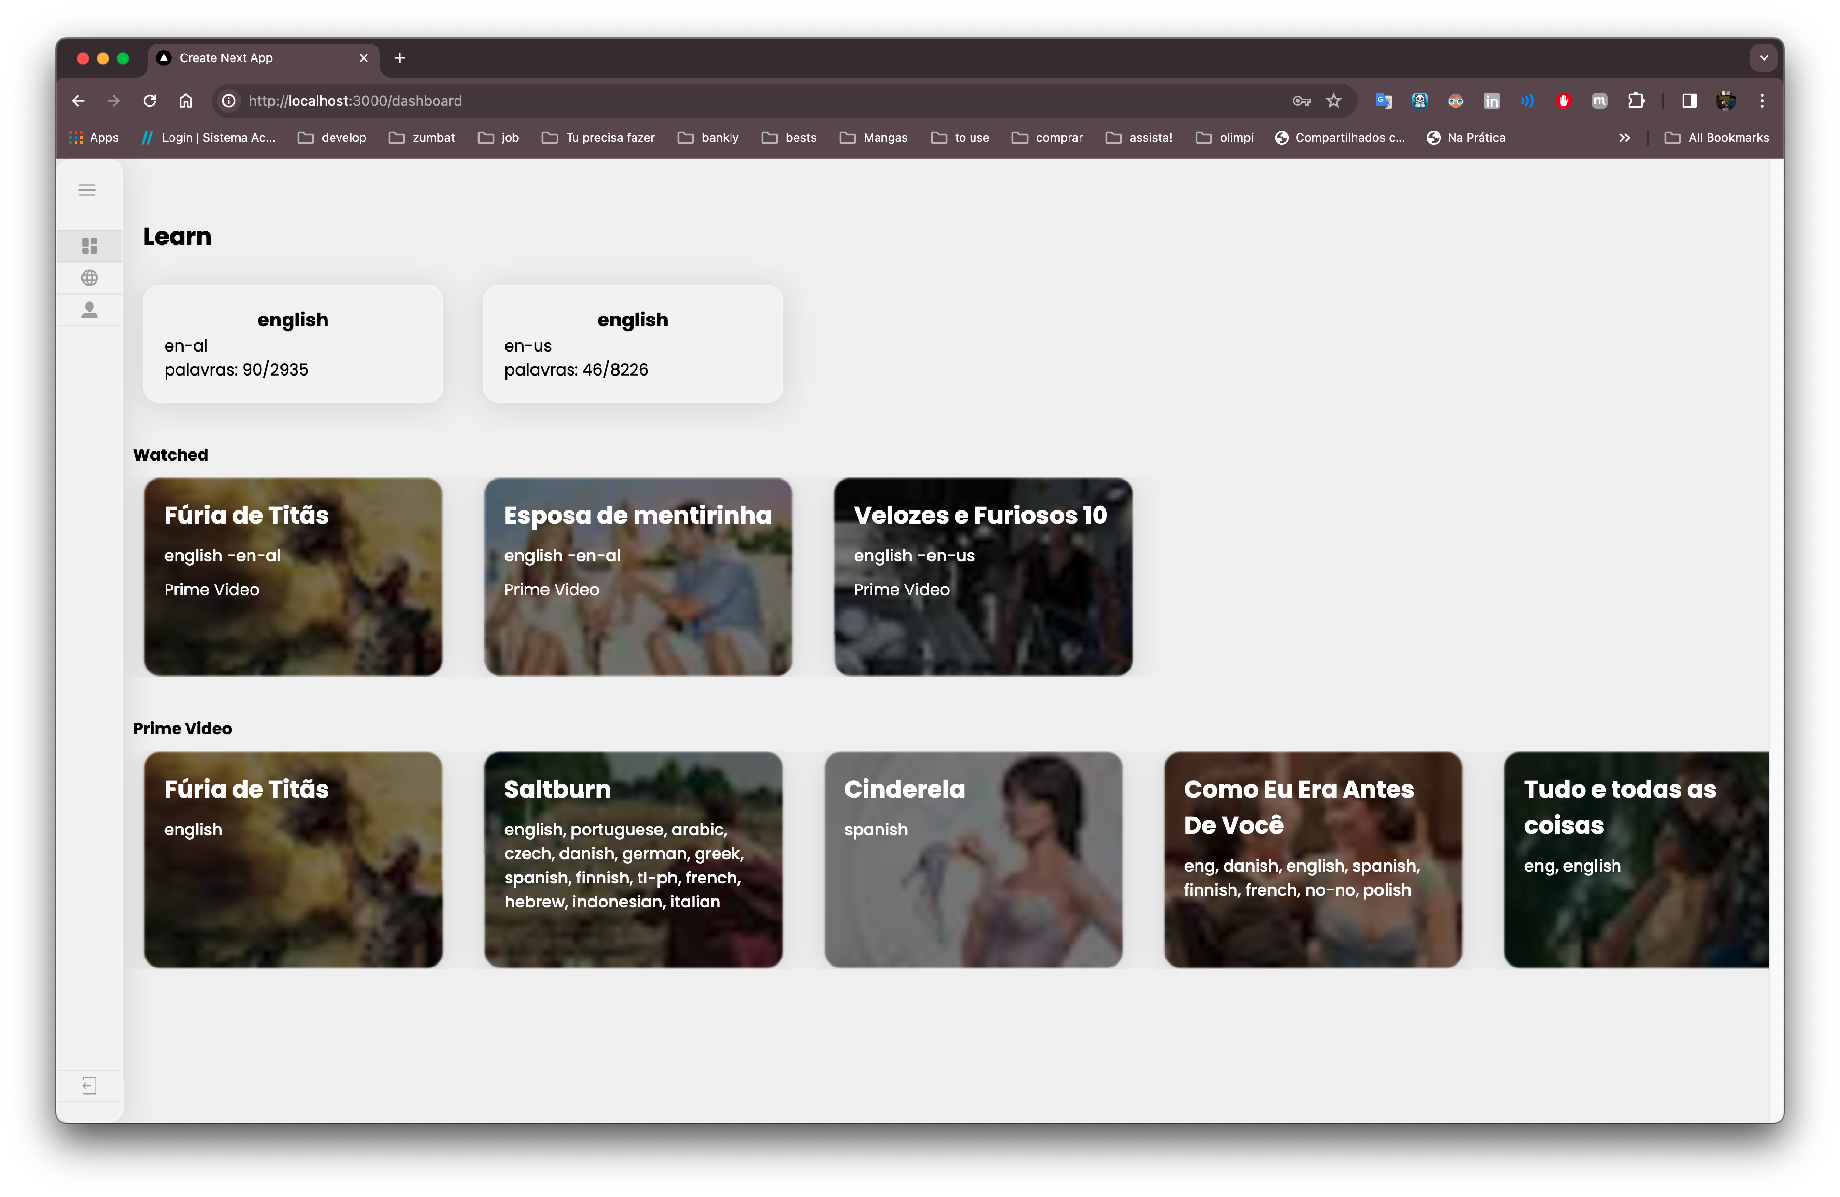
\includegraphics[width=0.8\textwidth]{assets/20.png}
  \end{figure}

  \begin{figure}
    \centering
    \caption{
    A list of languages that the user can learn. 
    }
    \label{fig:site2}
    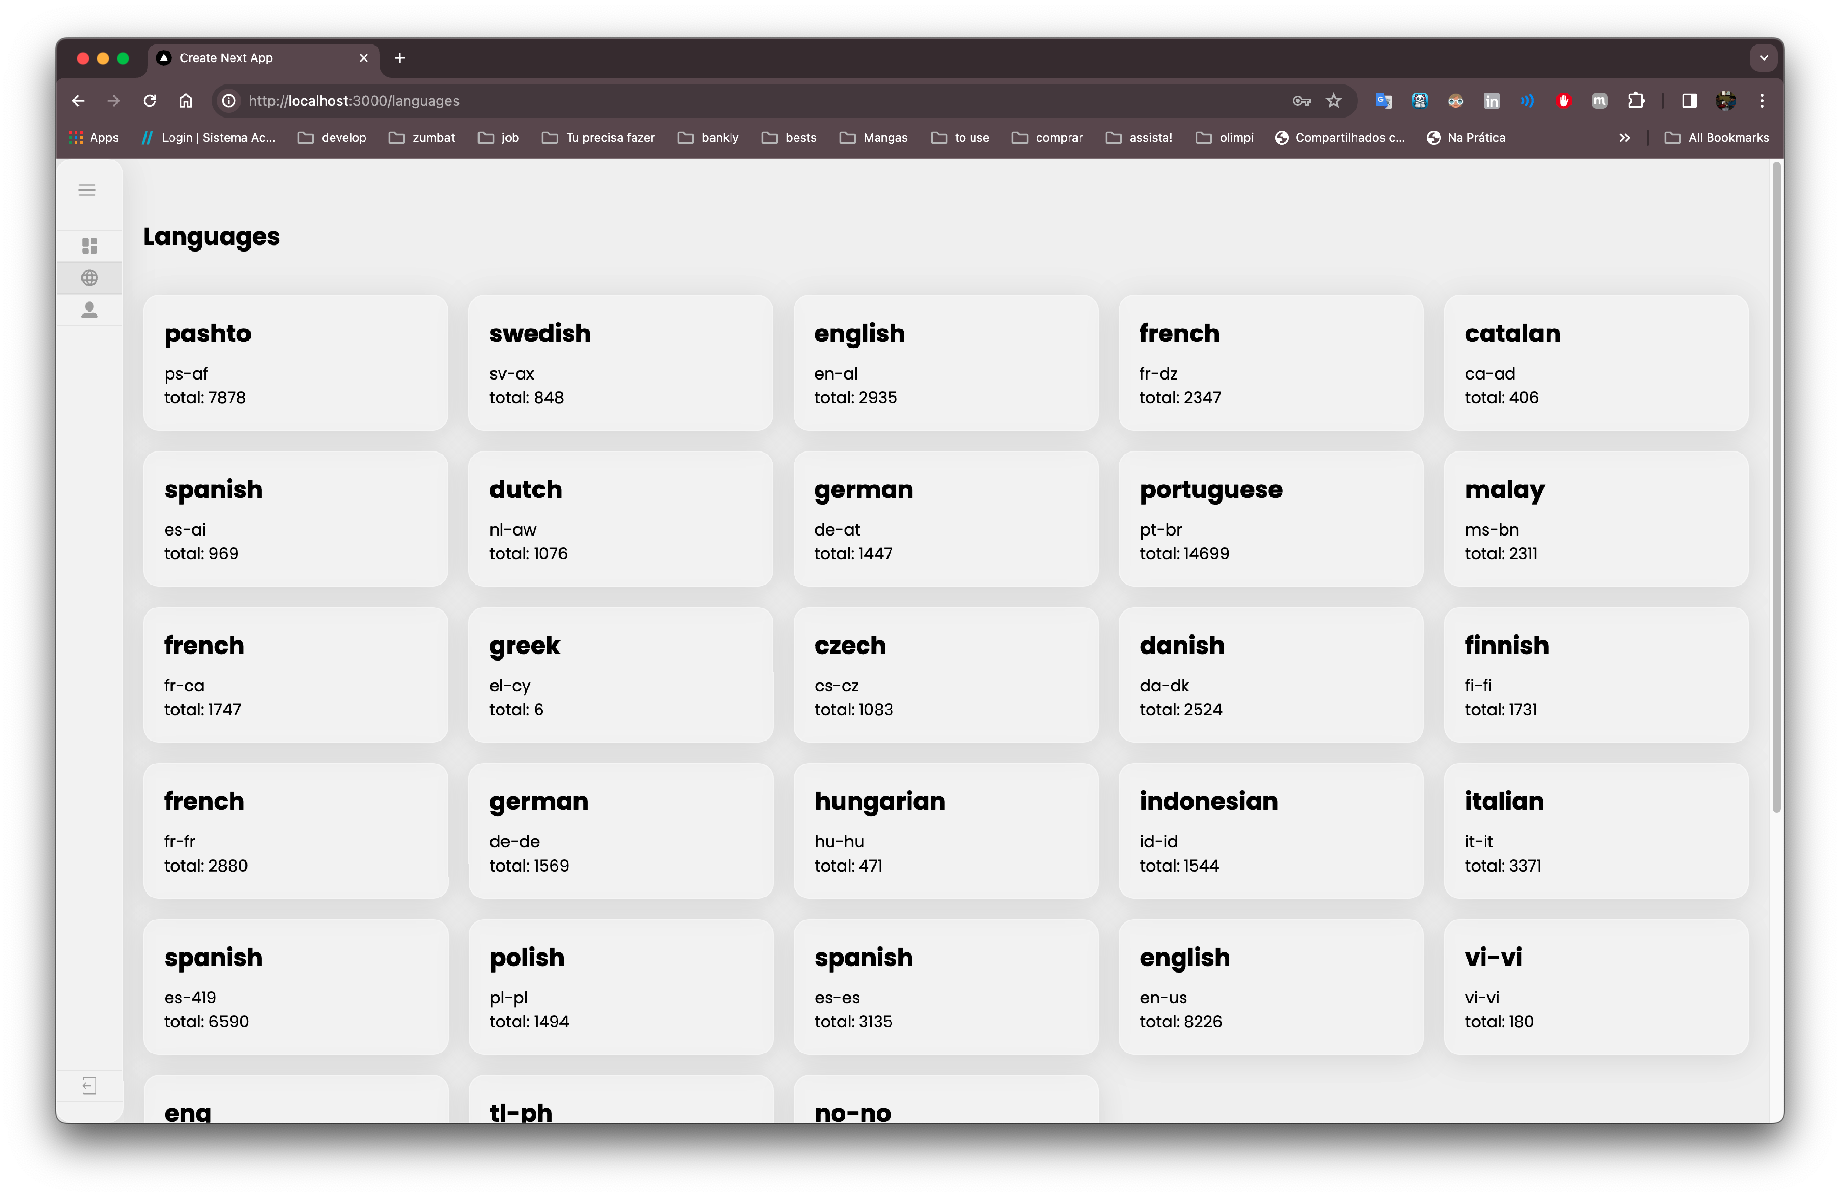
\includegraphics[width=0.8\textwidth]{assets/21.png}
  \end{figure}

    \begin{figure}
      \centering
      \caption{
      The user profile with progress for each language.
      }
      \label{fig:site3}
      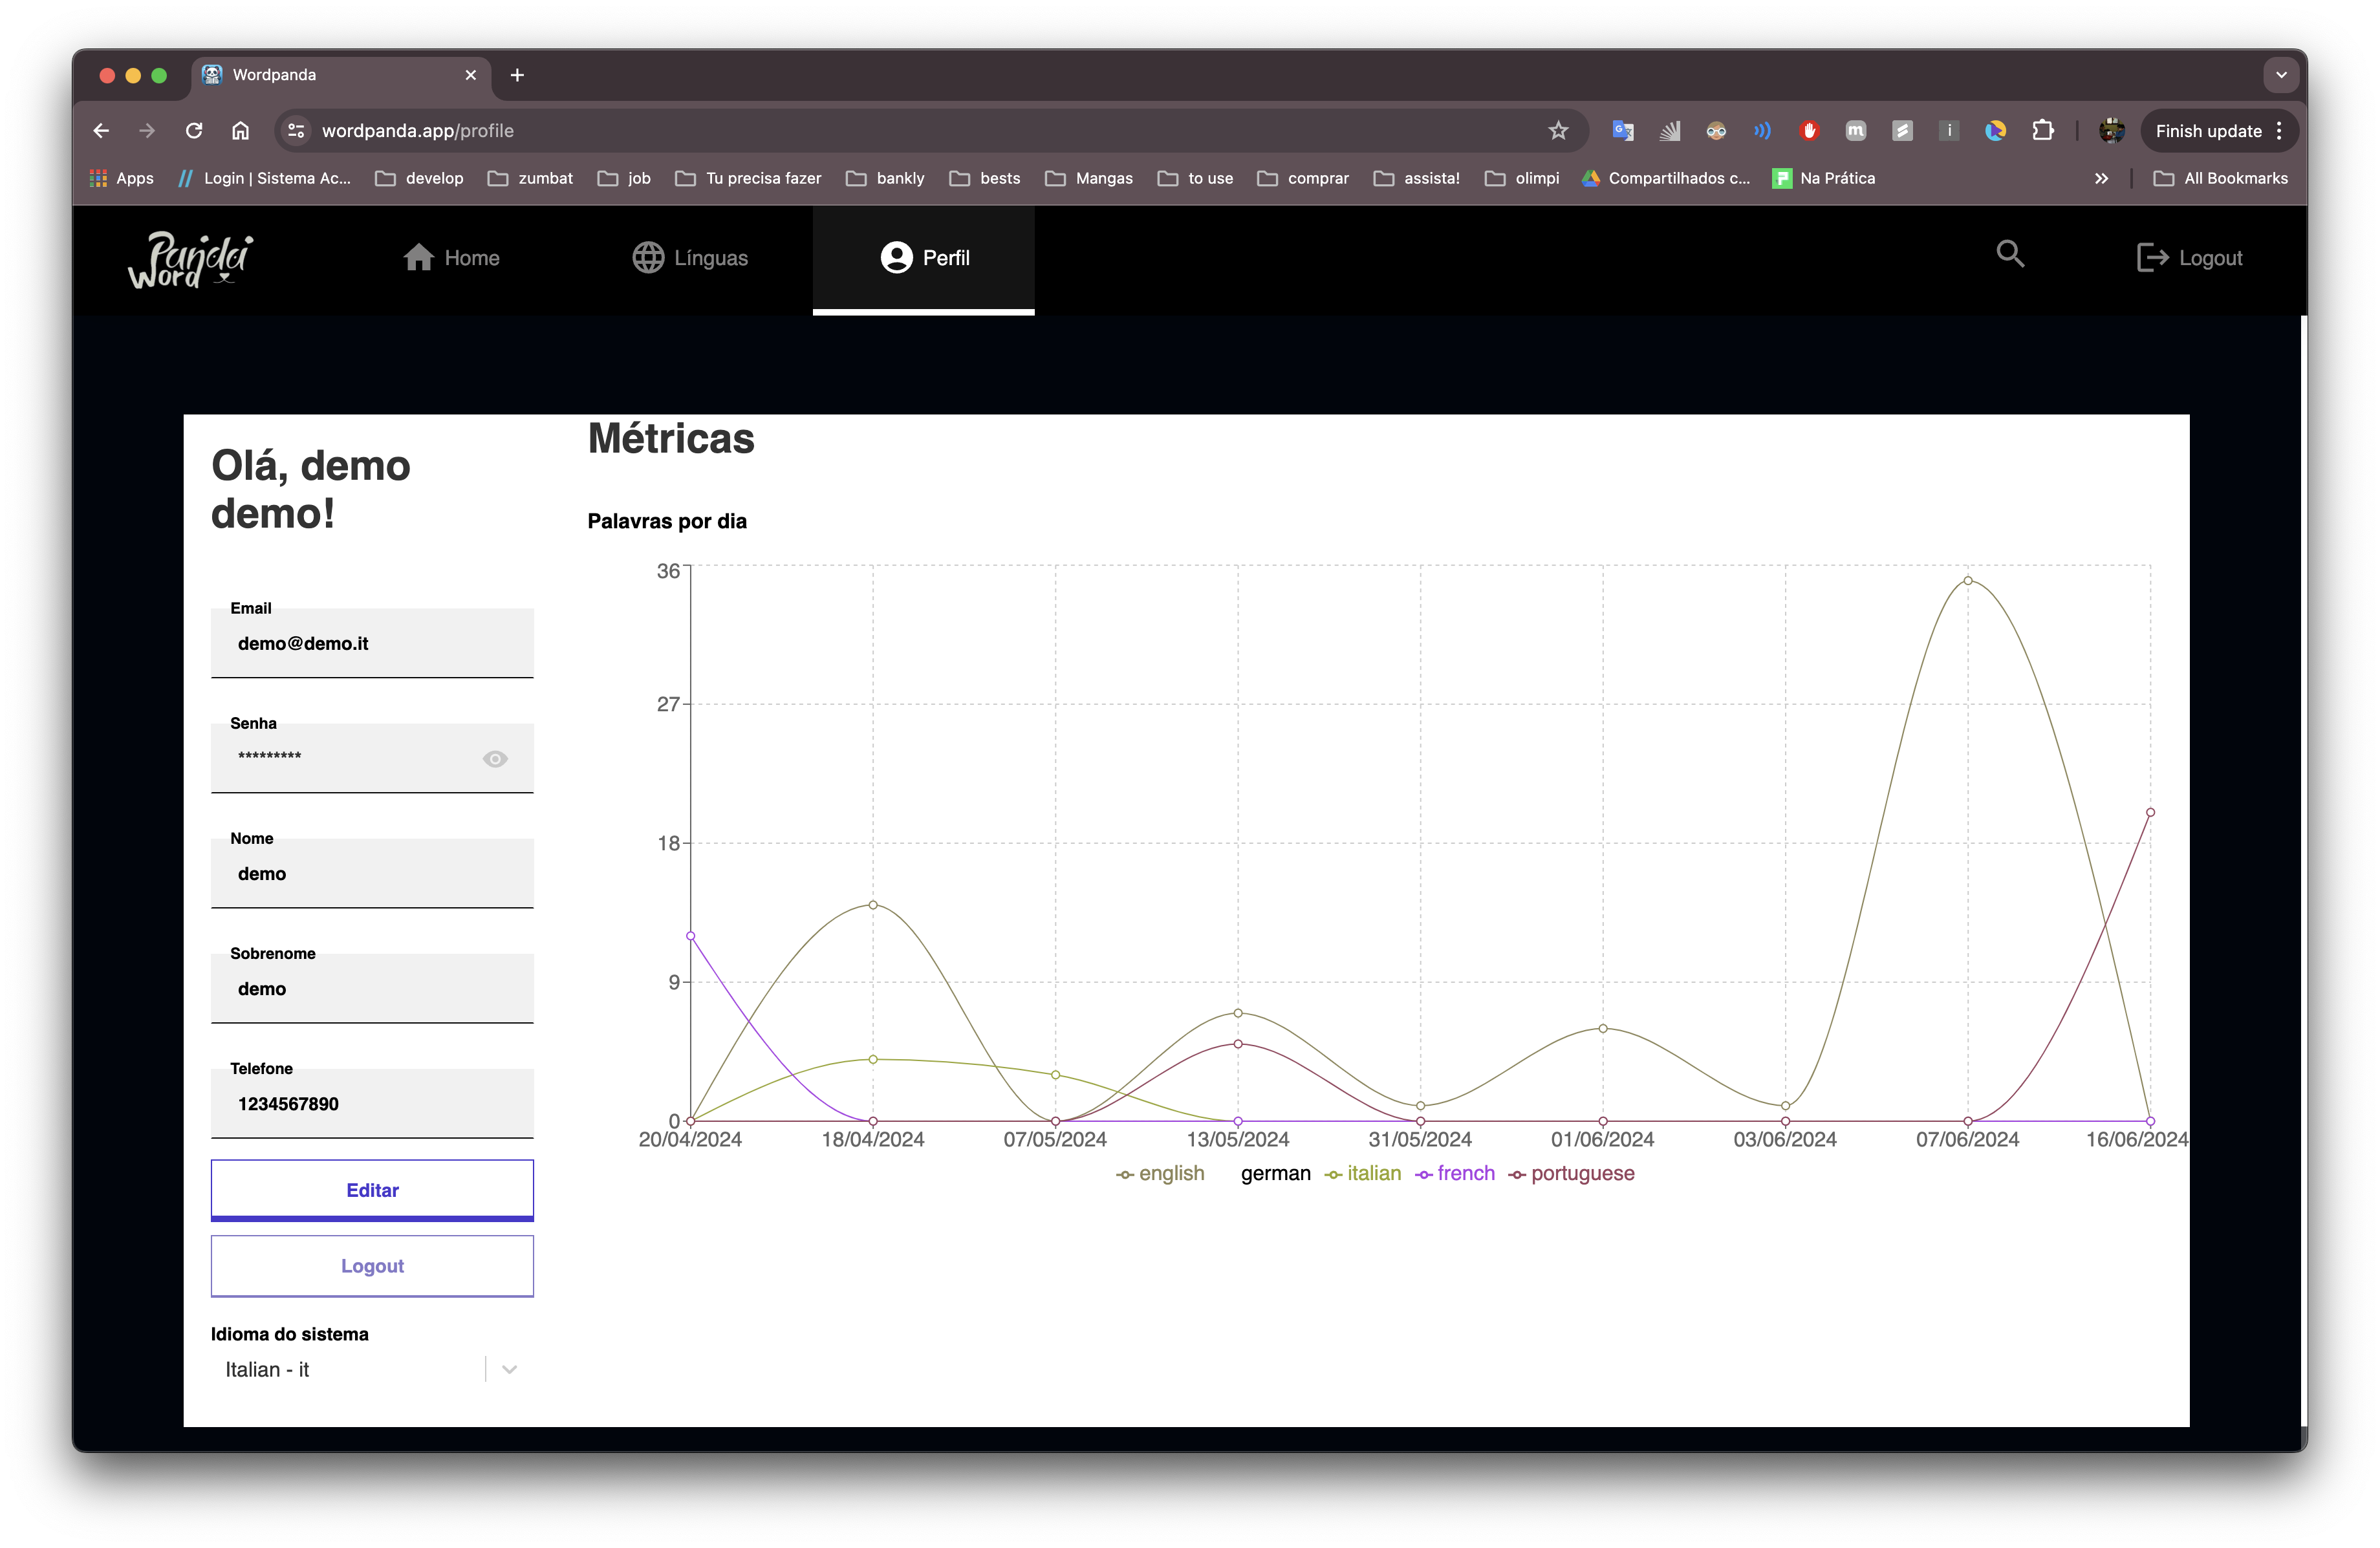
\includegraphics[width=0.8\textwidth]{assets/22.png}
    \end{figure}

    \begin{figure}
      \centering
      \caption{
      A list of languages when the user selects a language to learn.
      }
      \label{fig:site4}
      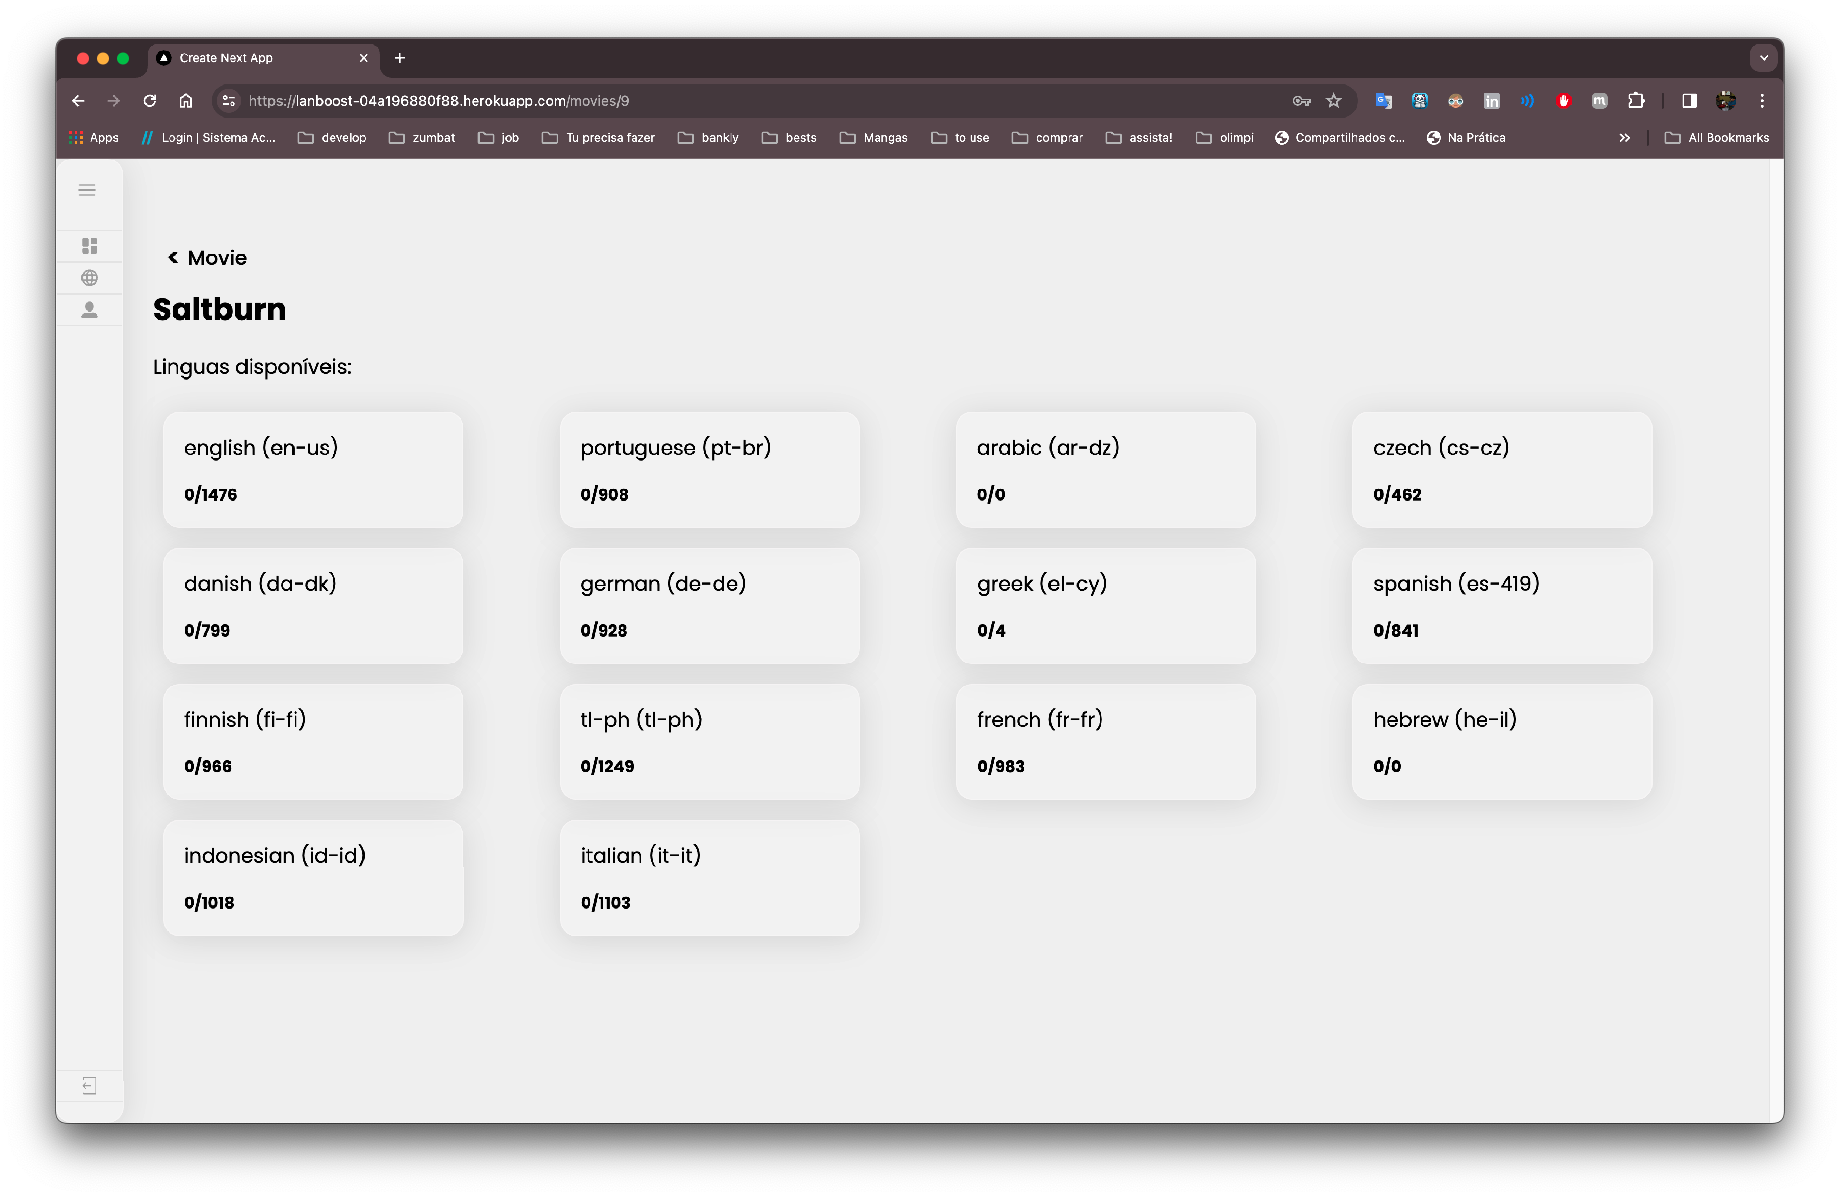
\includegraphics[width=0.8\textwidth]{assets/25.png}
    \end{figure}

    \begin{figure}
      \centering
      \caption{
      The possible games that the user can play.
      }
      \label{fig:site5}
      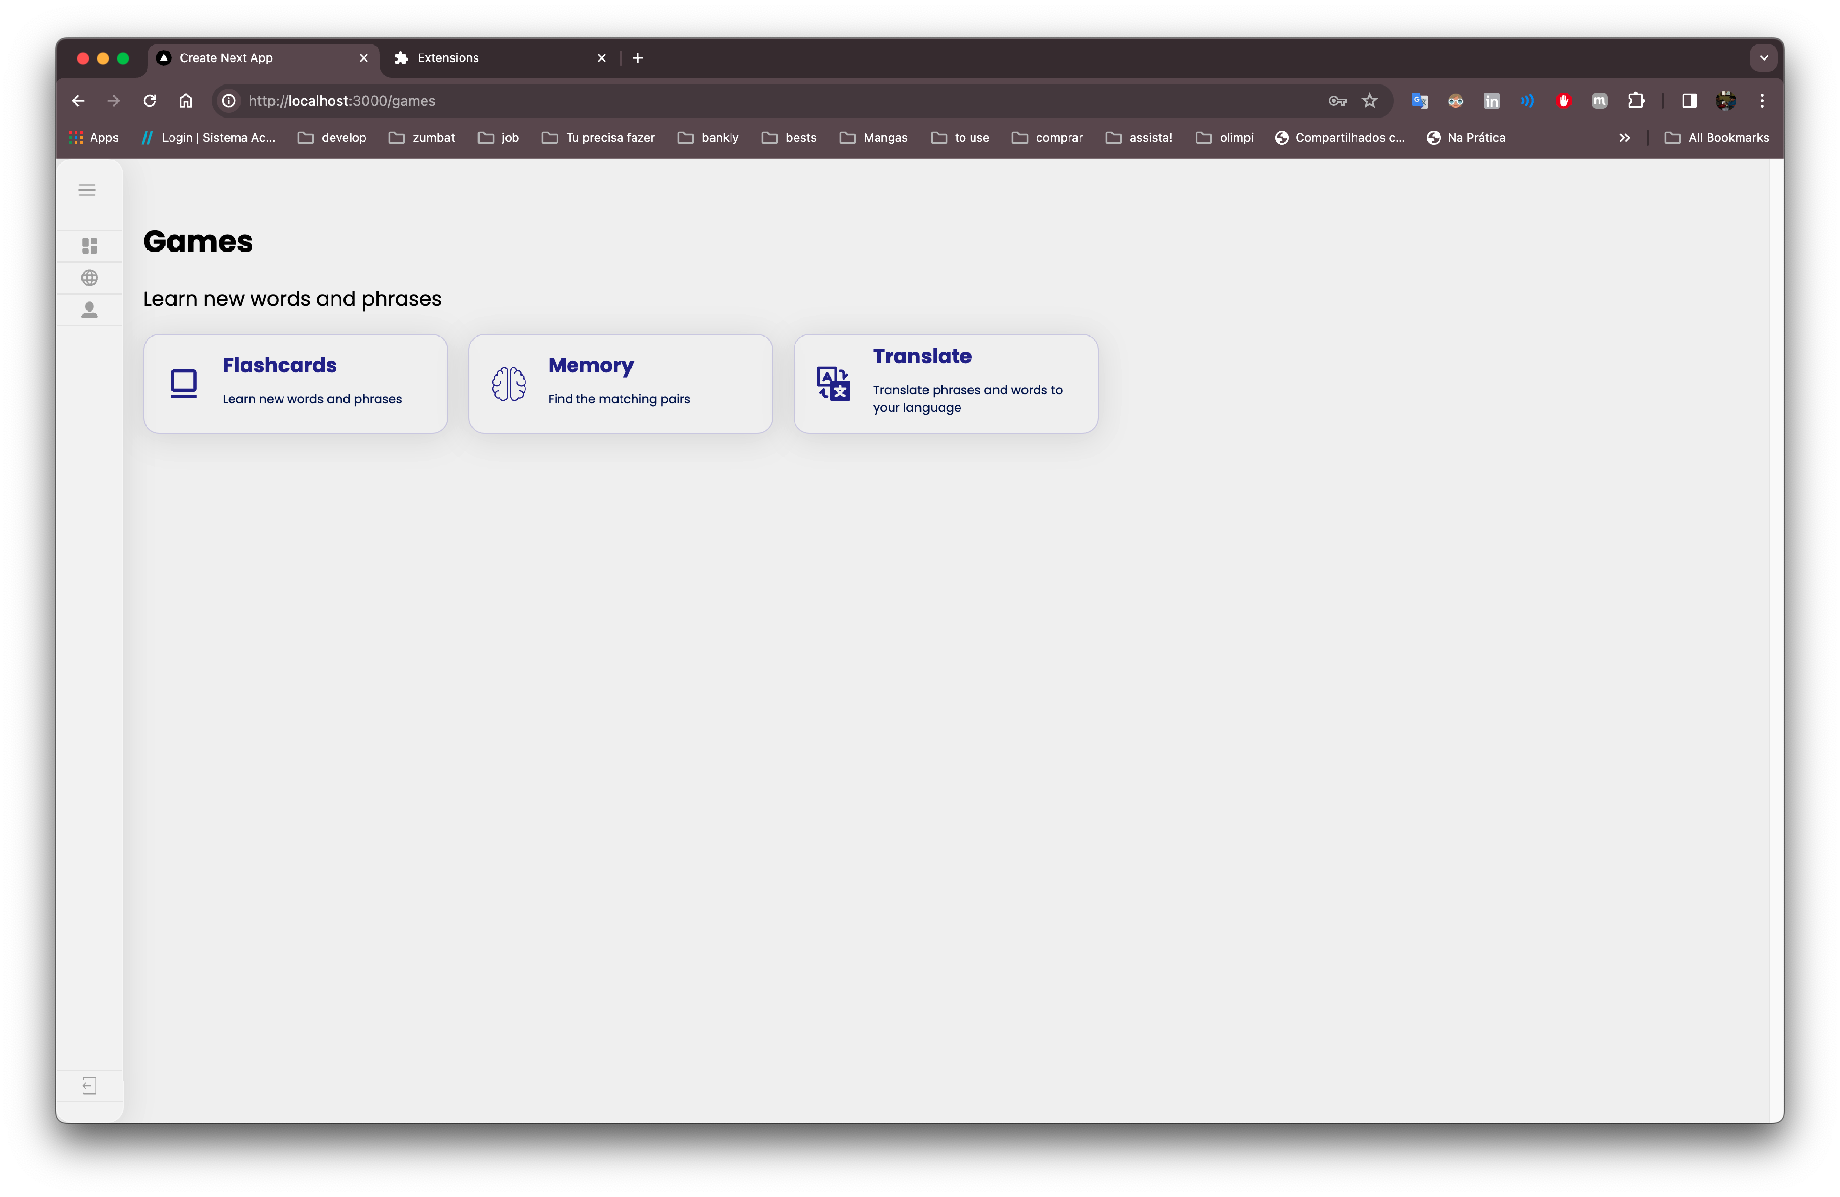
\includegraphics[width=0.8\textwidth]{assets/5.png}
    \end{figure}


    \begin{figure}
      \centering
      \caption{
      Example of the flashcard game 
      }
      \label{fig:site6}
      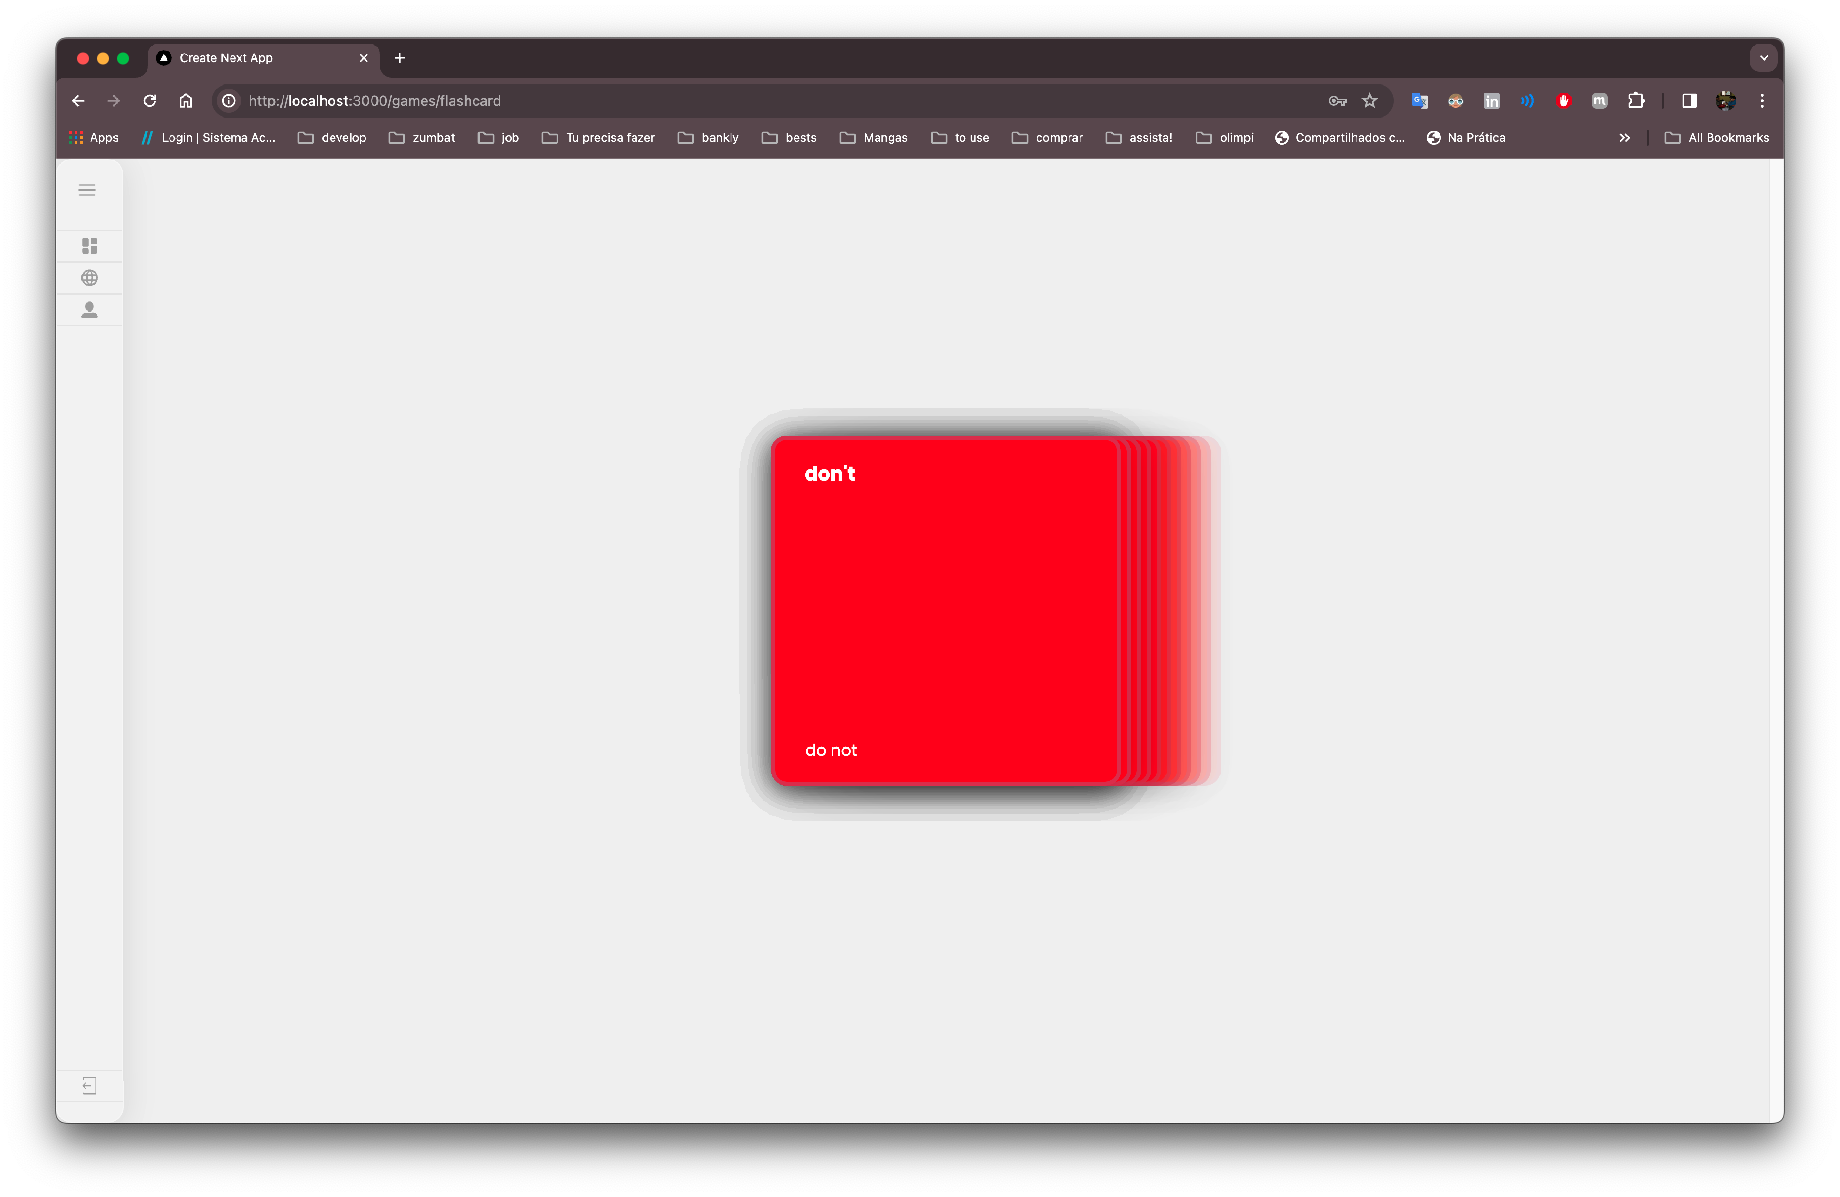
\includegraphics[width=0.8\textwidth]{assets/6.png}
    \end{figure}


    \begin{figure}
      \centering
      \caption{
      Example of the Memory game 
      }
      \label{fig:site7}
      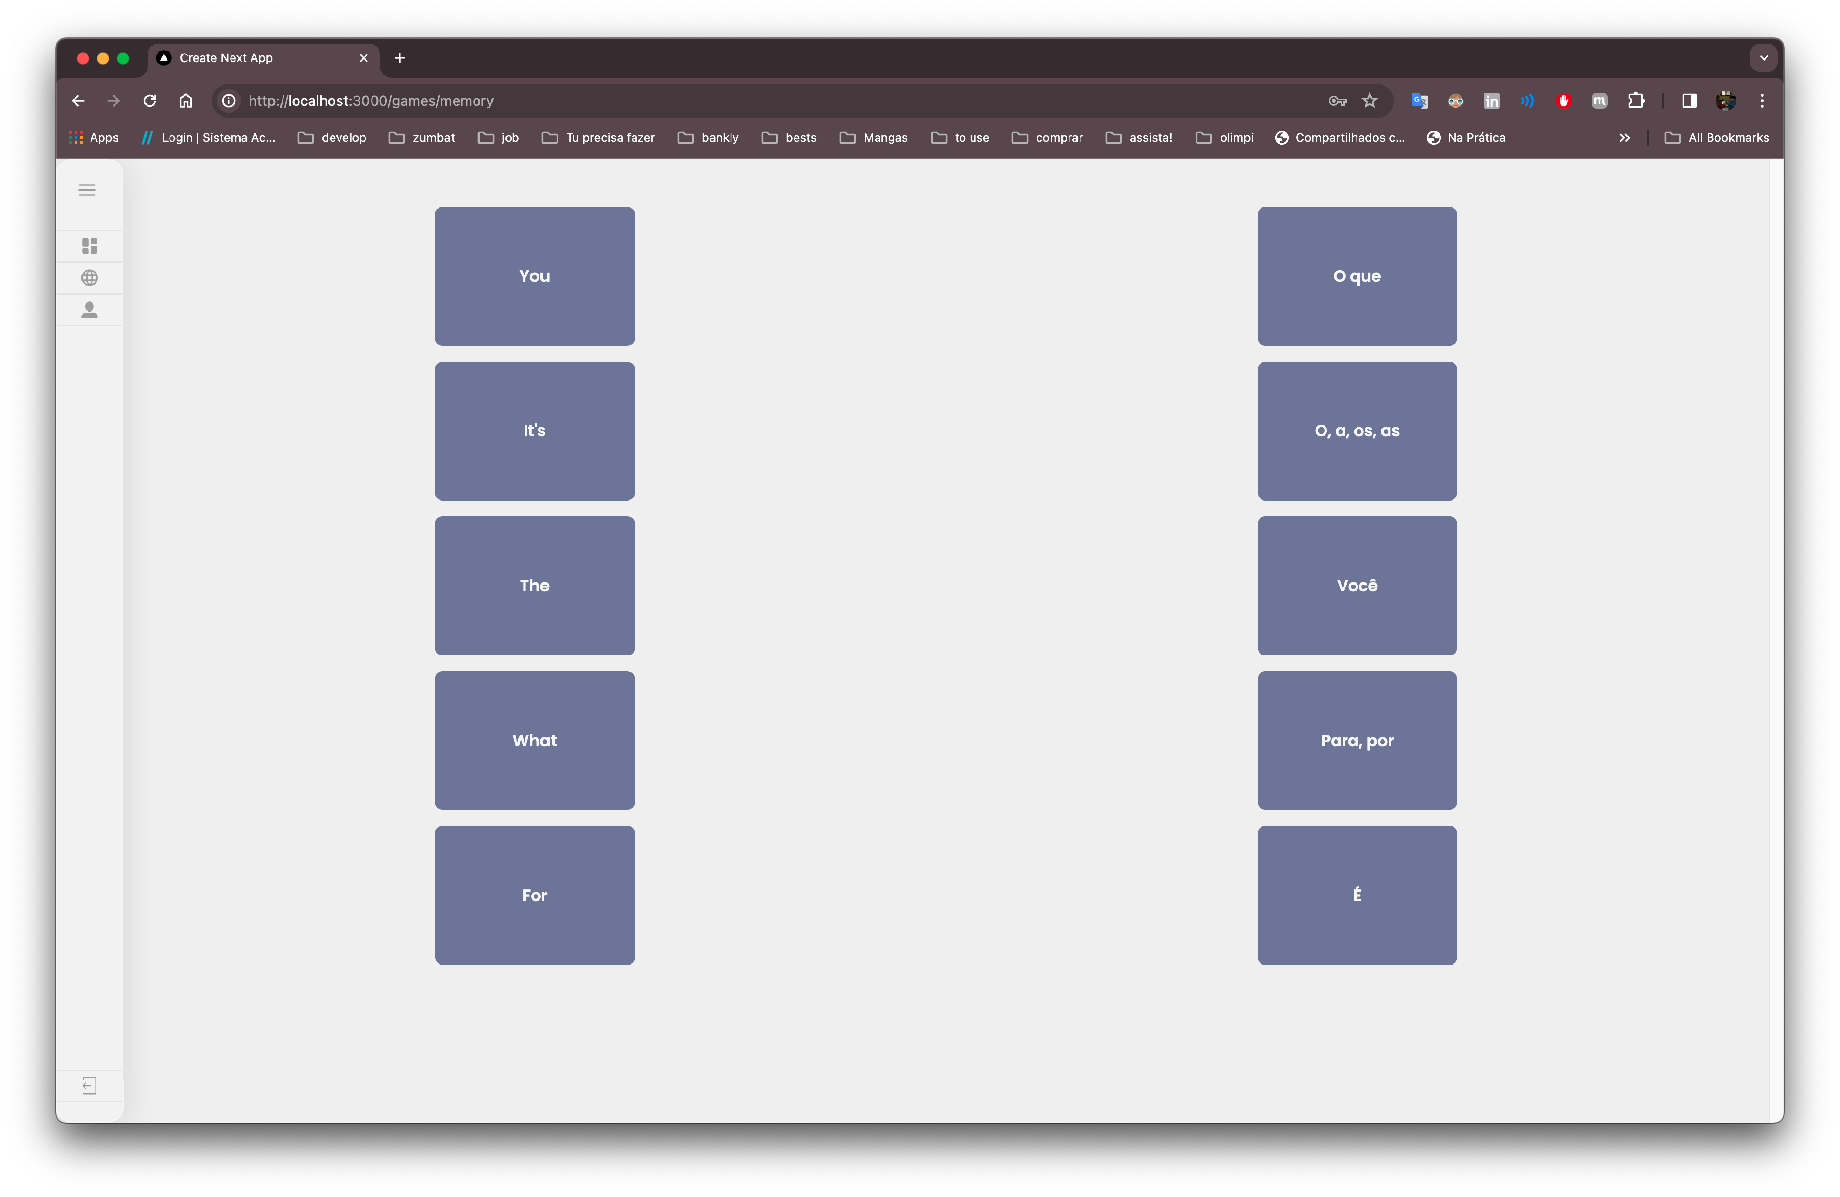
\includegraphics[width=0.8\textwidth]{assets/7.png}
    \end{figure}

    \begin{figure}
      \centering
      \caption{
      Example of the Quiz game 
      }
      \label{fig:site8}
      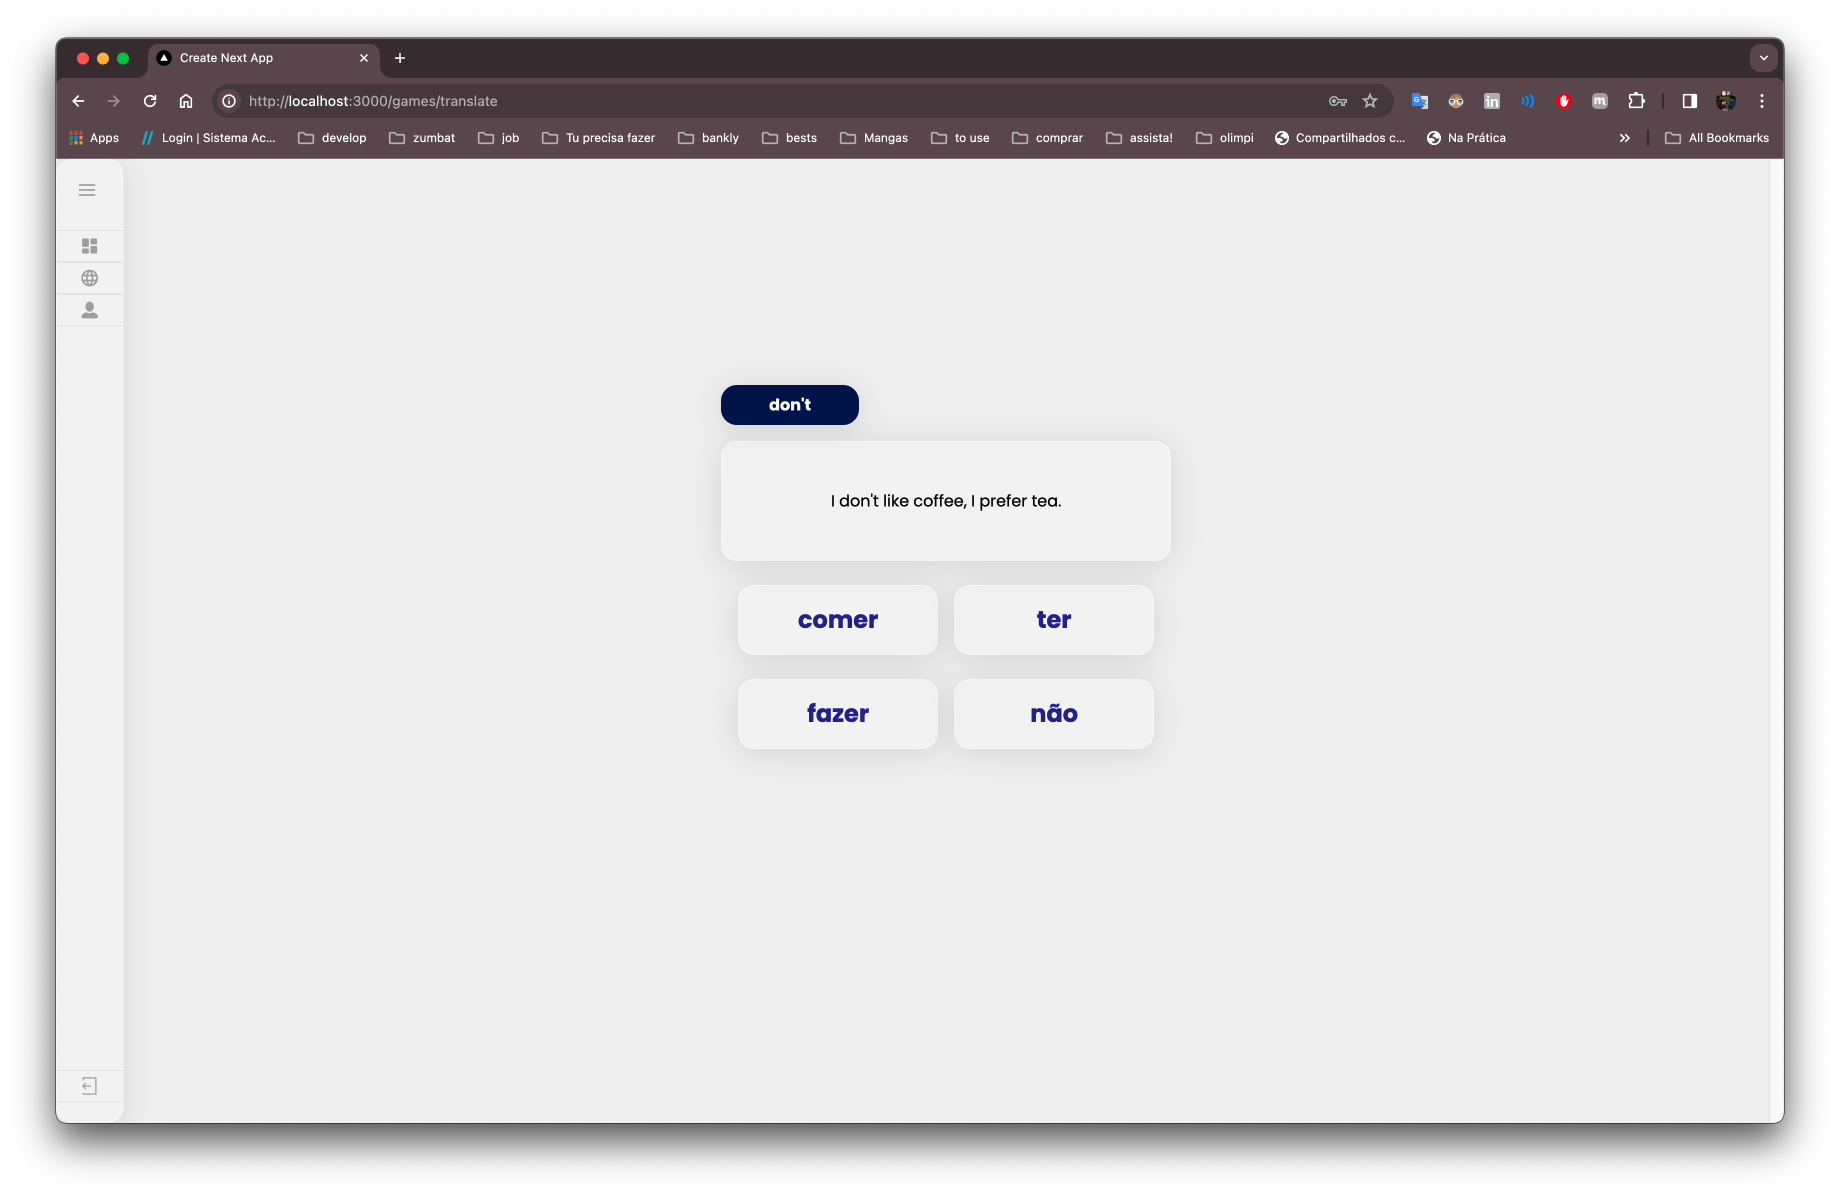
\includegraphics[width=0.8\textwidth]{assets/8.png}
    \end{figure}


    The iframe inserted on the browser was the interface of:

    \begin{itemize}
    \item The list of games that the user can play, as demonstrated in the figure-\ref{fig:iframe1}.
    \item The Flashcard, Memory and Quiz games, as demonstrated in the figure-\ref{fig:iframe2}, figure-\ref{fig:iframe3}, and figure-\ref{fig:iframe4}.
    \end{itemize}


    \begin{figure}
      \centering
      \caption{
      Games list inside iframe on the prime video site.
      }
      \label{fig:iframe1}
      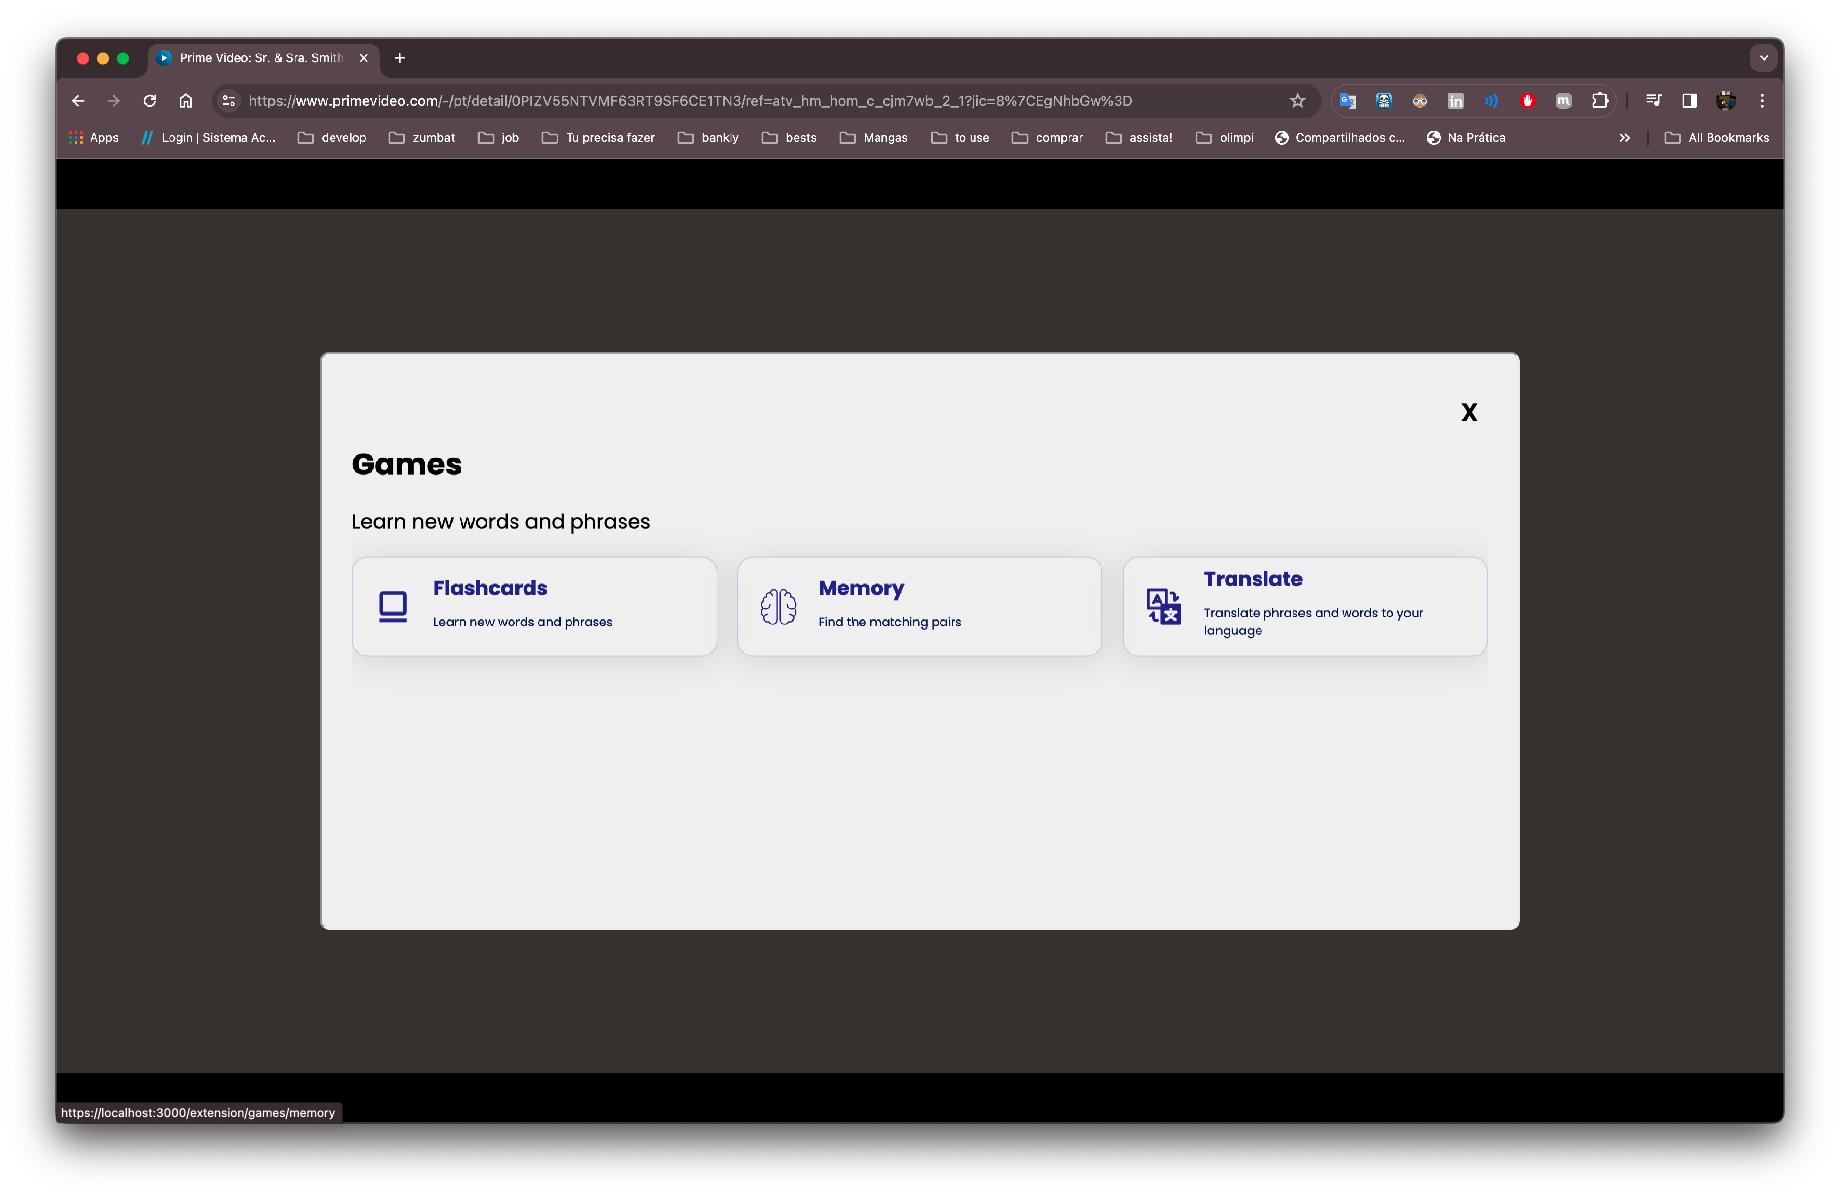
\includegraphics[width=0.8\textwidth]{assets/9.png}
    \end{figure}

    \begin{figure}
      \centering
      \caption{
      Games Flashcard inside iframe on the prime video site.
      }
      \label{fig:iframe2}
      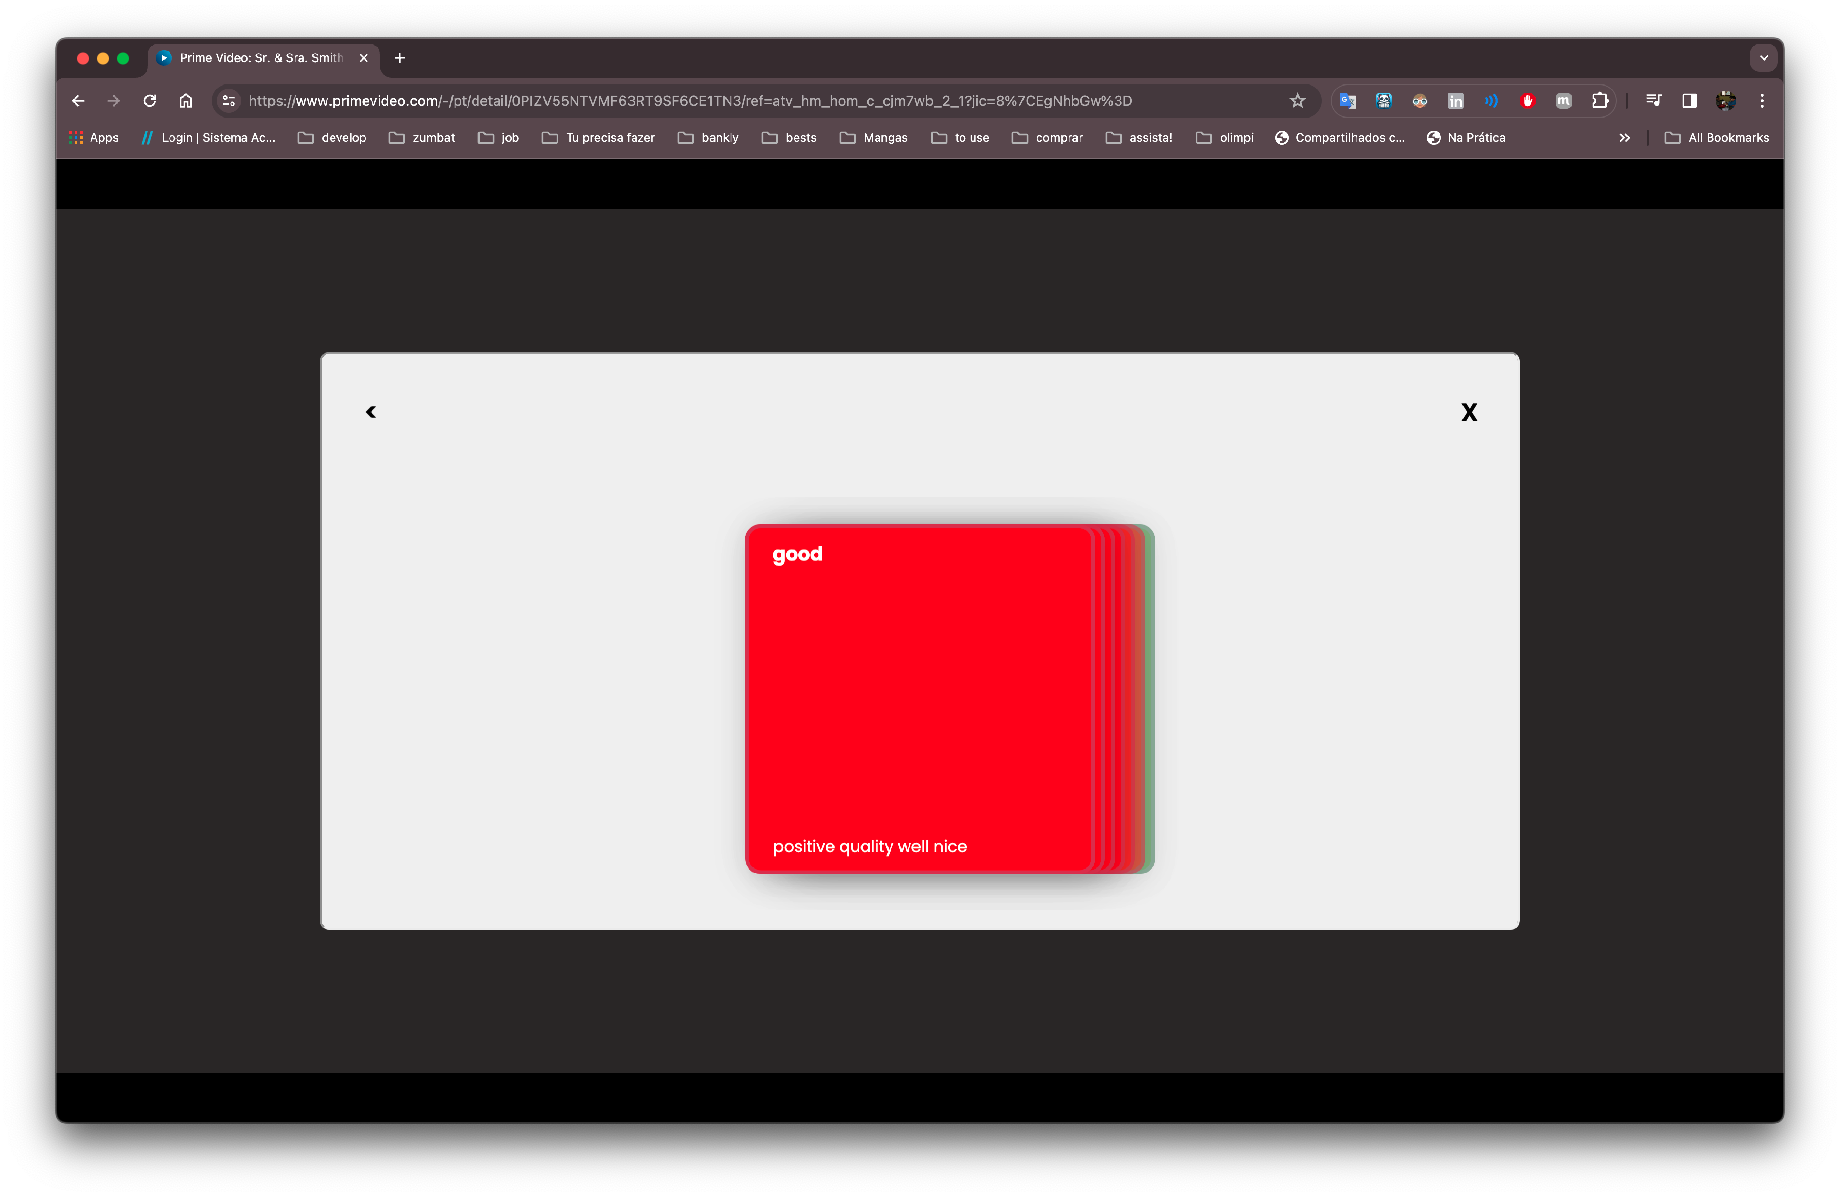
\includegraphics[width=0.8\textwidth]{assets/10.png}
    \end{figure}

    \begin{figure}
      \centering
      \caption{
      Games Memory inside iframe on the prime video site.
      }
      \label{fig:iframe3}
      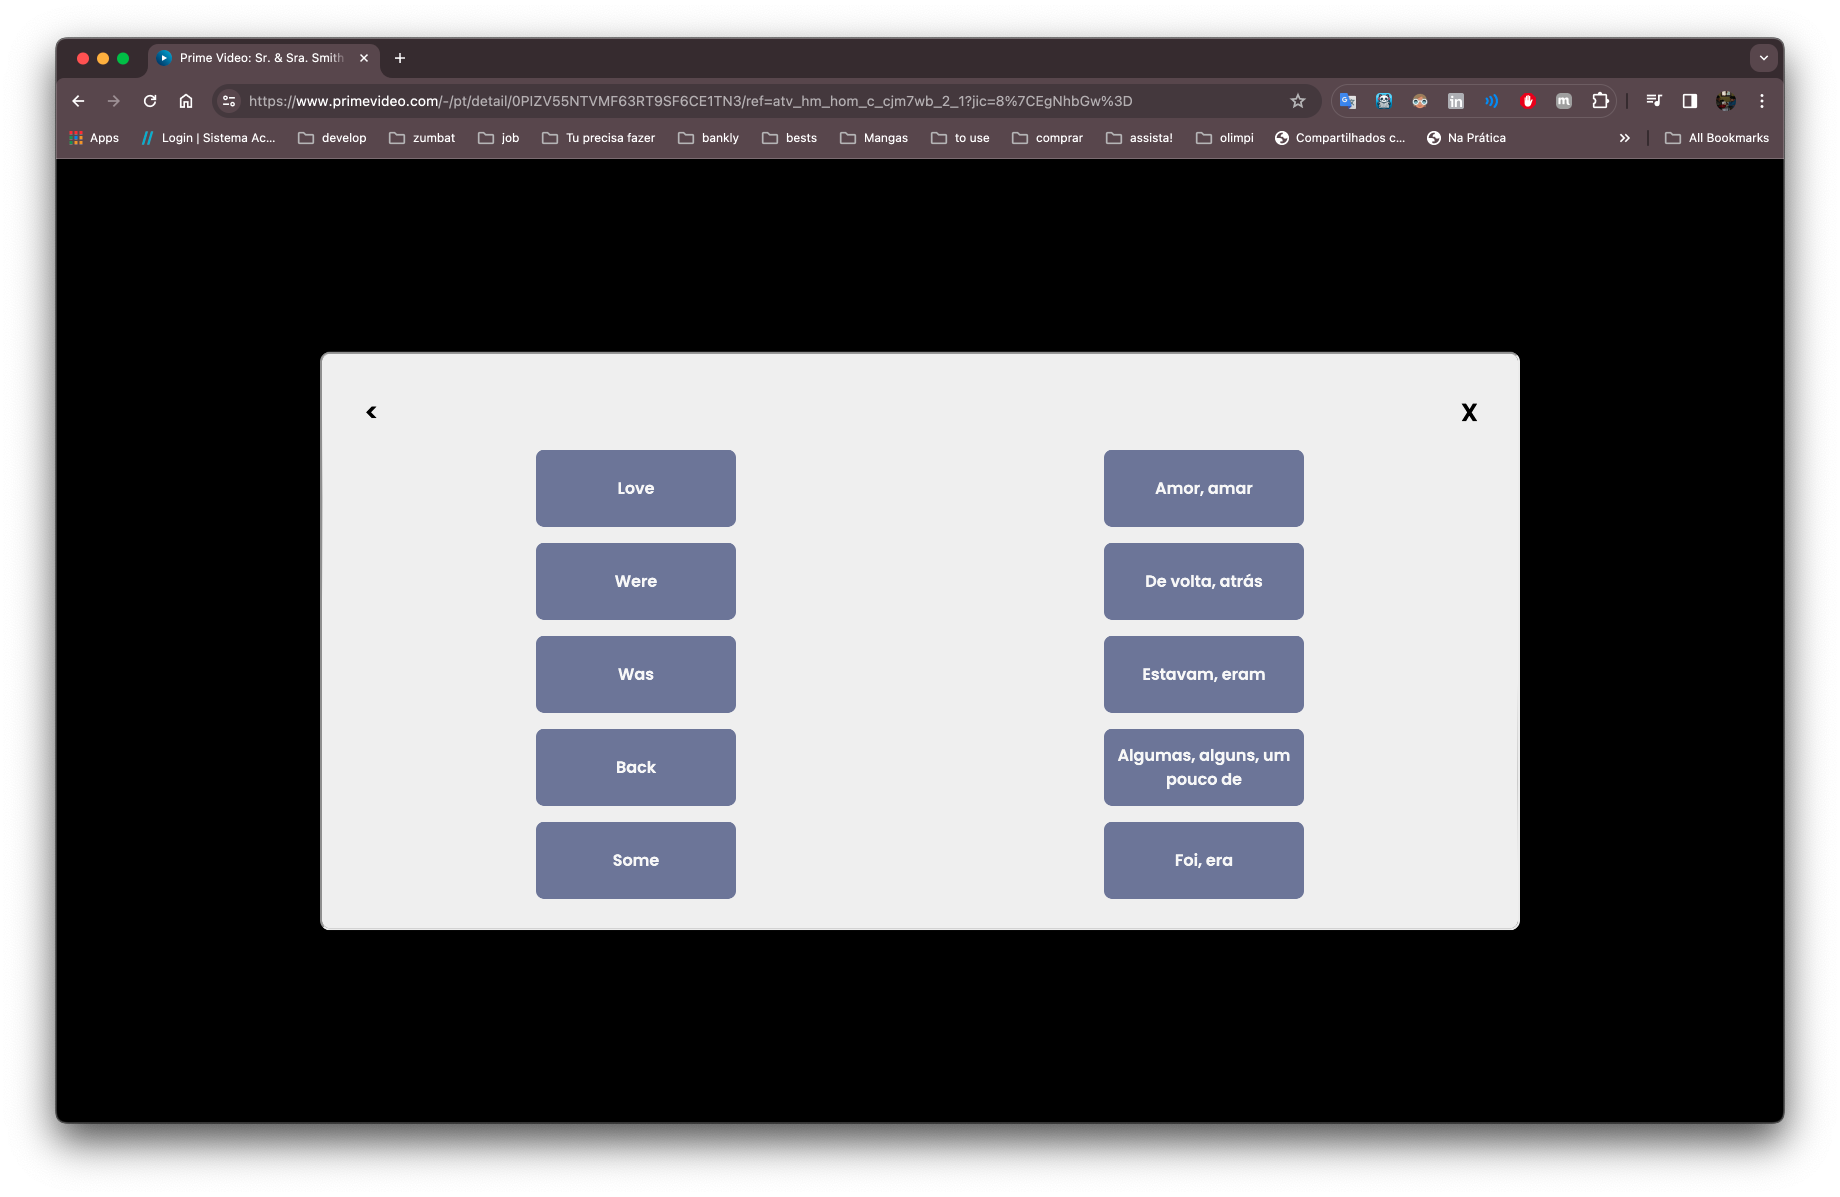
\includegraphics[width=0.8\textwidth]{assets/11.png}
    \end{figure}

    \begin{figure}
      \centering
      \caption{
      Games Translate inside iframe on the prime video site.
      }
      \label{fig:iframe4}
      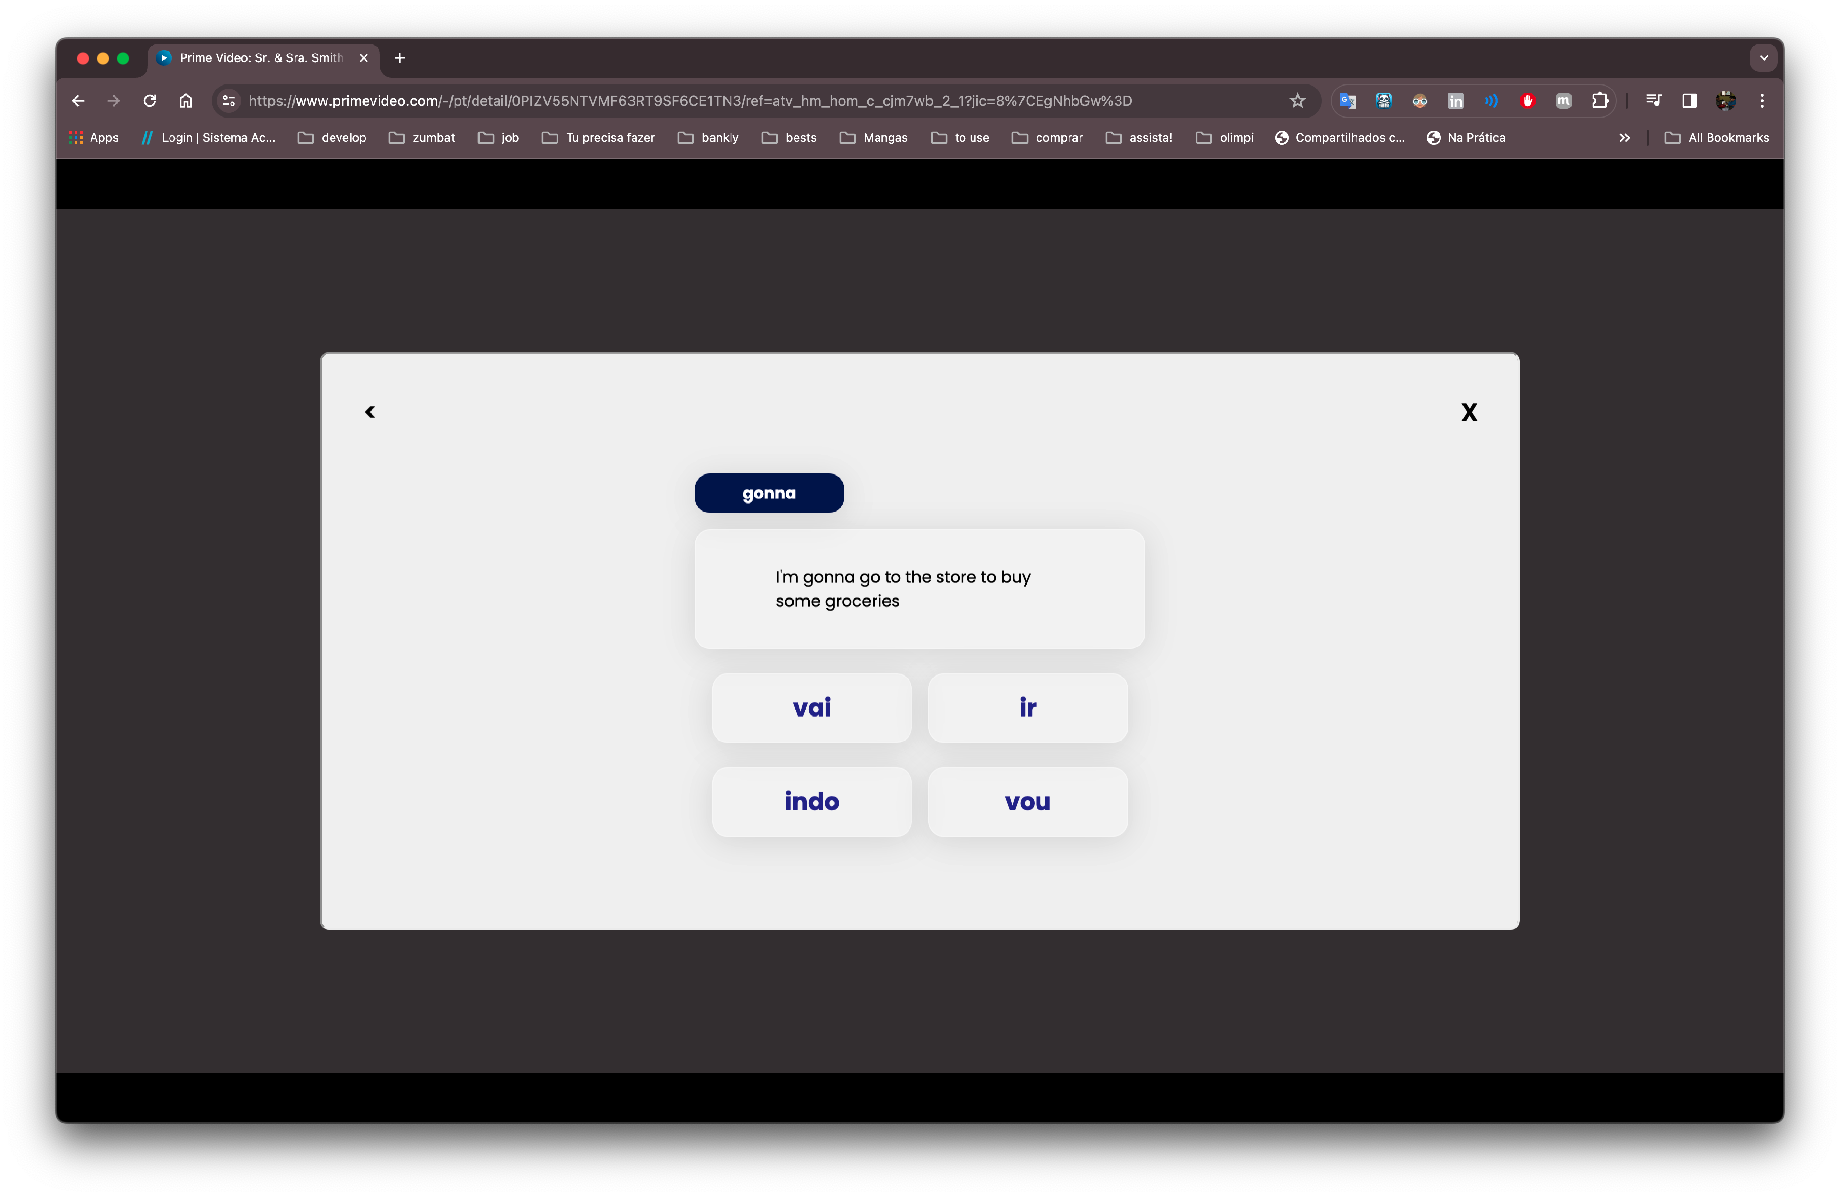
\includegraphics[width=0.8\textwidth]{assets/12.png}
    \end{figure}



The app iframe was the interface of:

\begin{itemize}
  \item login as demonstrated in the figure-\ref{fig:app1}.
  \item List of languages and movies as demonstrated in the figure-\ref{fig:app2}.
  \item List of languages as demonstrated in the figure-\ref{fig:app3}.
  \item List of languages by movie as demonstrated in the figure-\ref{fig:app4} and figure-\ref{fig:app5}.
  \item Translate game as demonstrated in the figure-\ref{fig:app6}.
  \item And the others games as the site and iframe extension. 
  \end{itemize}



  \begin{figure}
    \centering
    \caption{
    Login inside iframe on the app.
    }
    \label{fig:app1}
    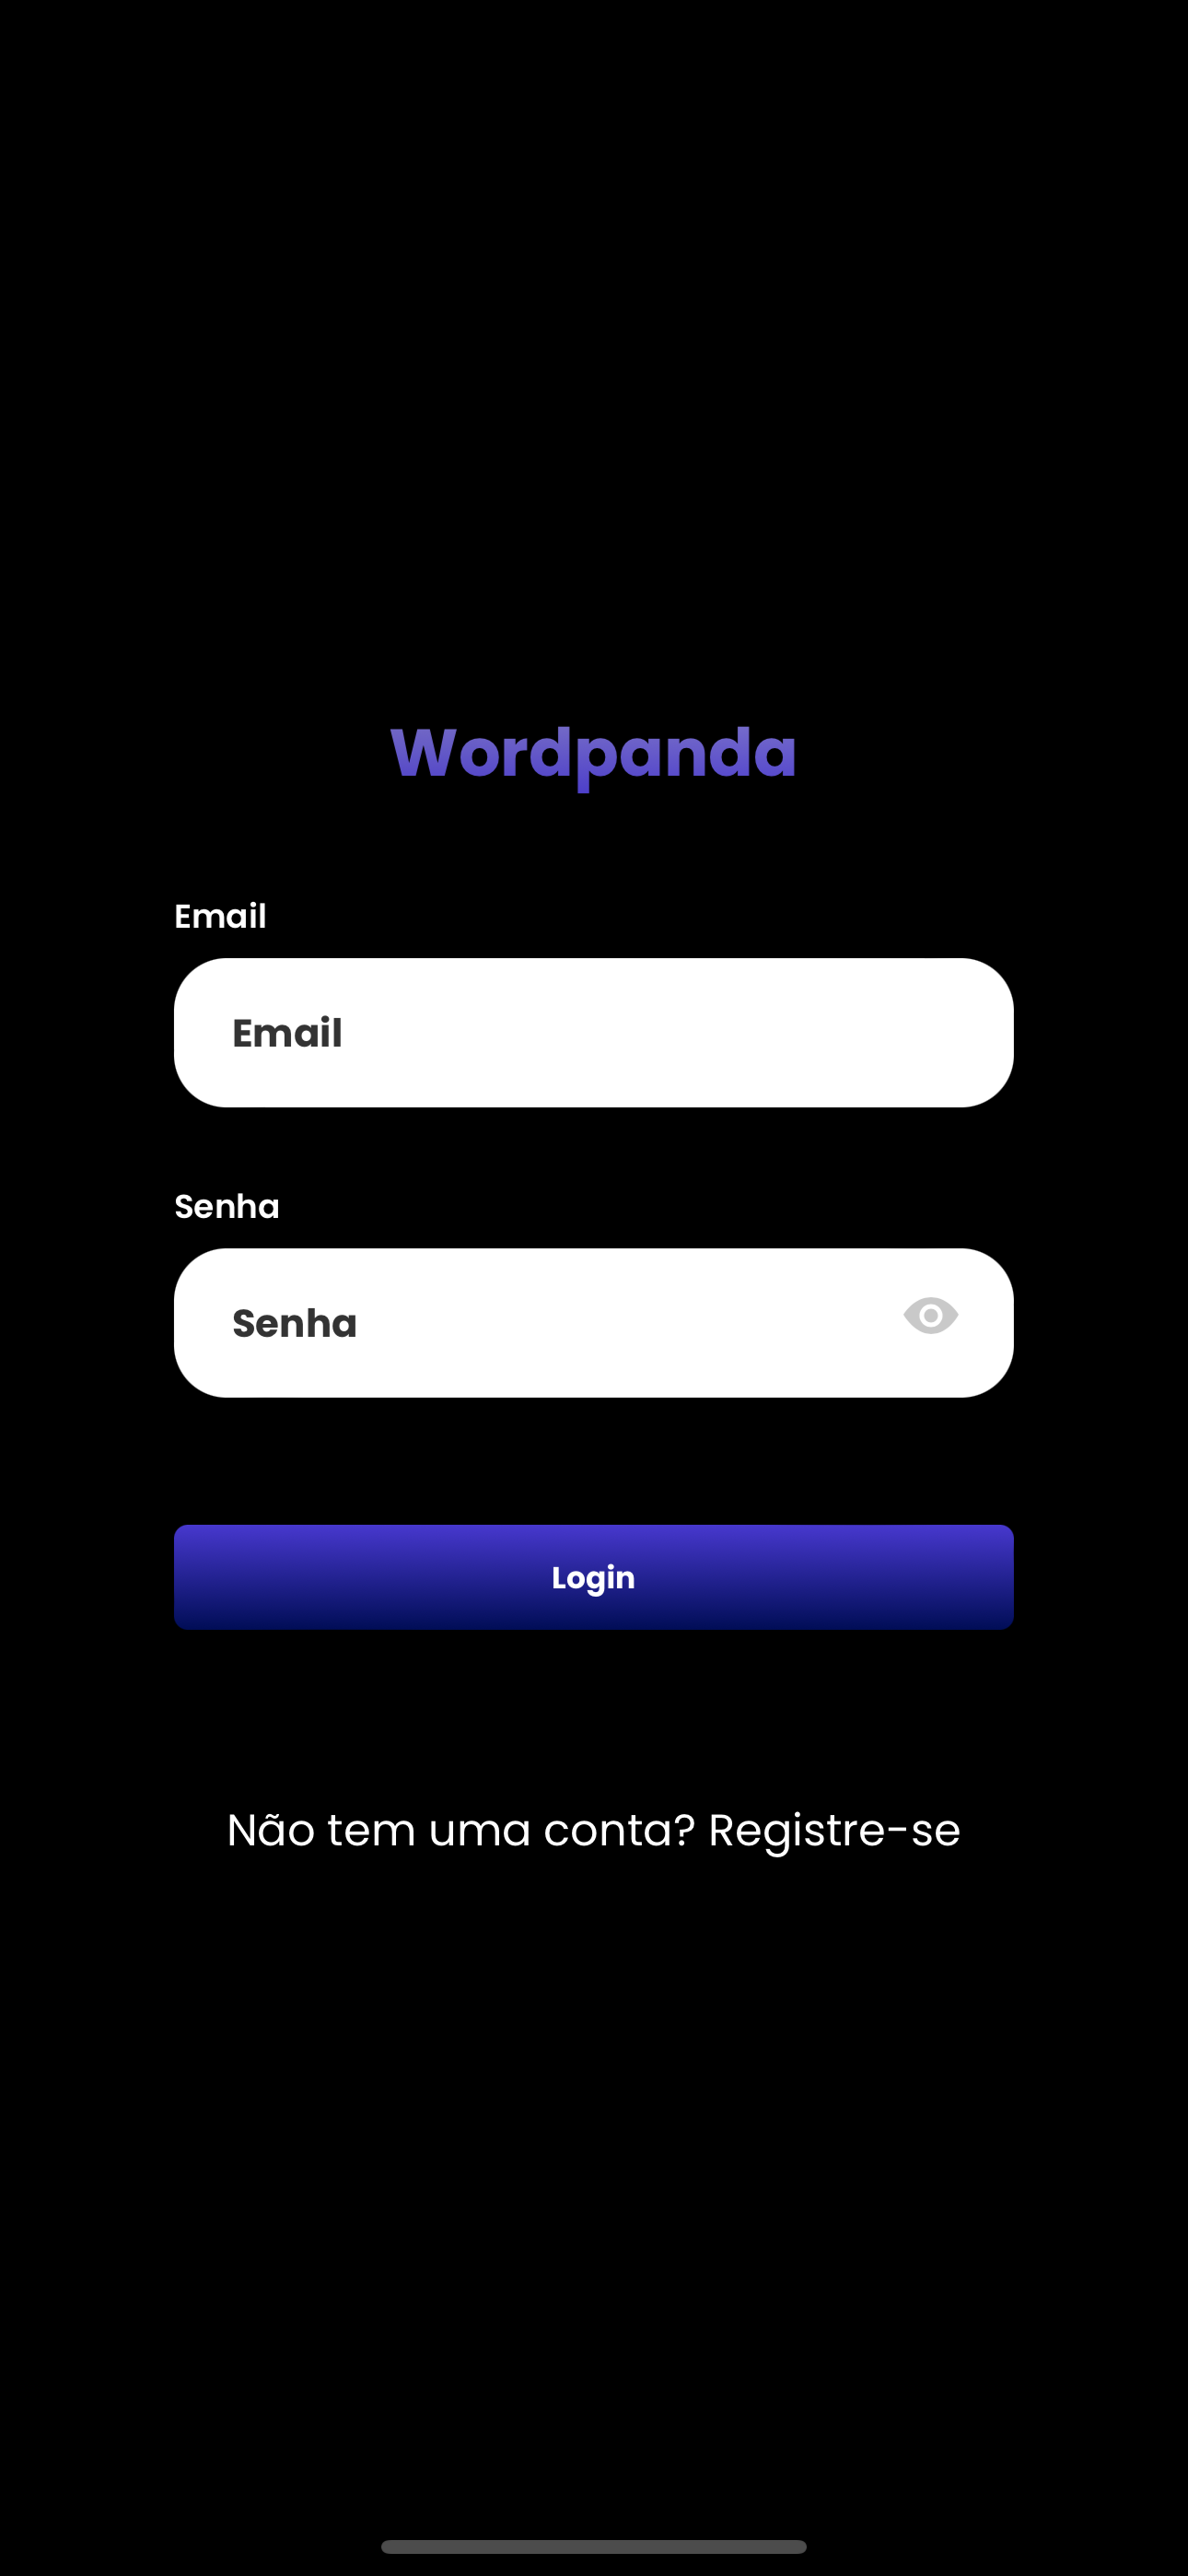
\includegraphics[width=0.4\textwidth]{assets/14.png}
  \end{figure}

  \begin{figure}
    \centering
    \caption{
     List of languages and movies inside iframe on the app.
    }
    \label{fig:app2}
    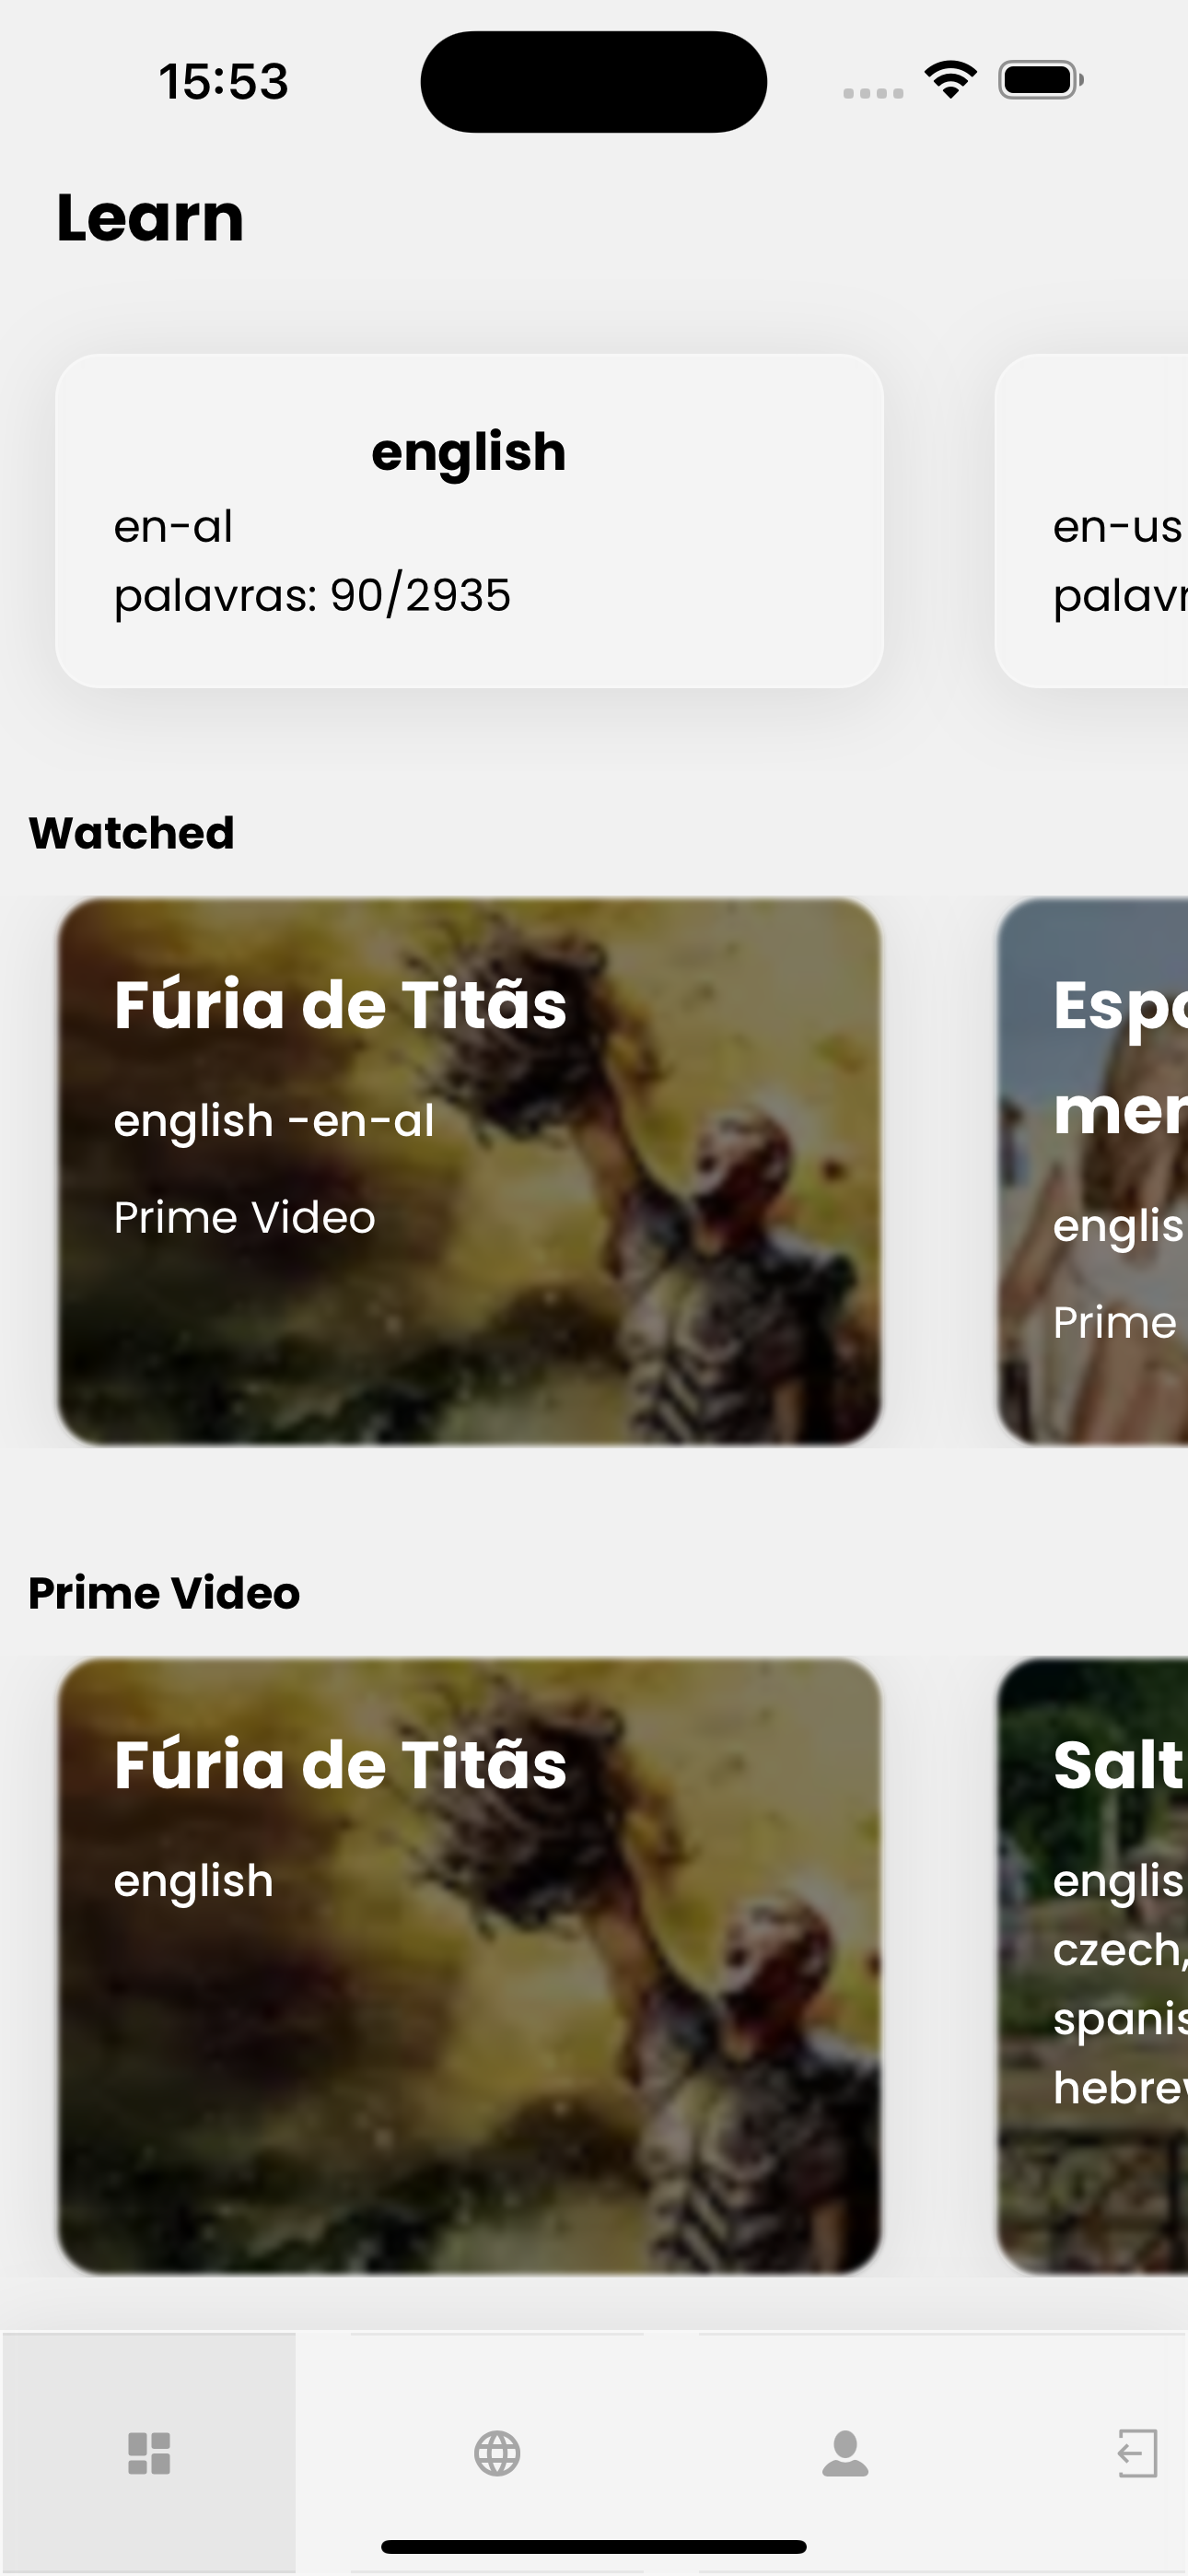
\includegraphics[width=0.4\textwidth]{assets/15.png}
  \end{figure}

  \begin{figure}
    \centering
    \caption{
     List of languages inside iframe on the app.
    }
    \label{fig:app3}
    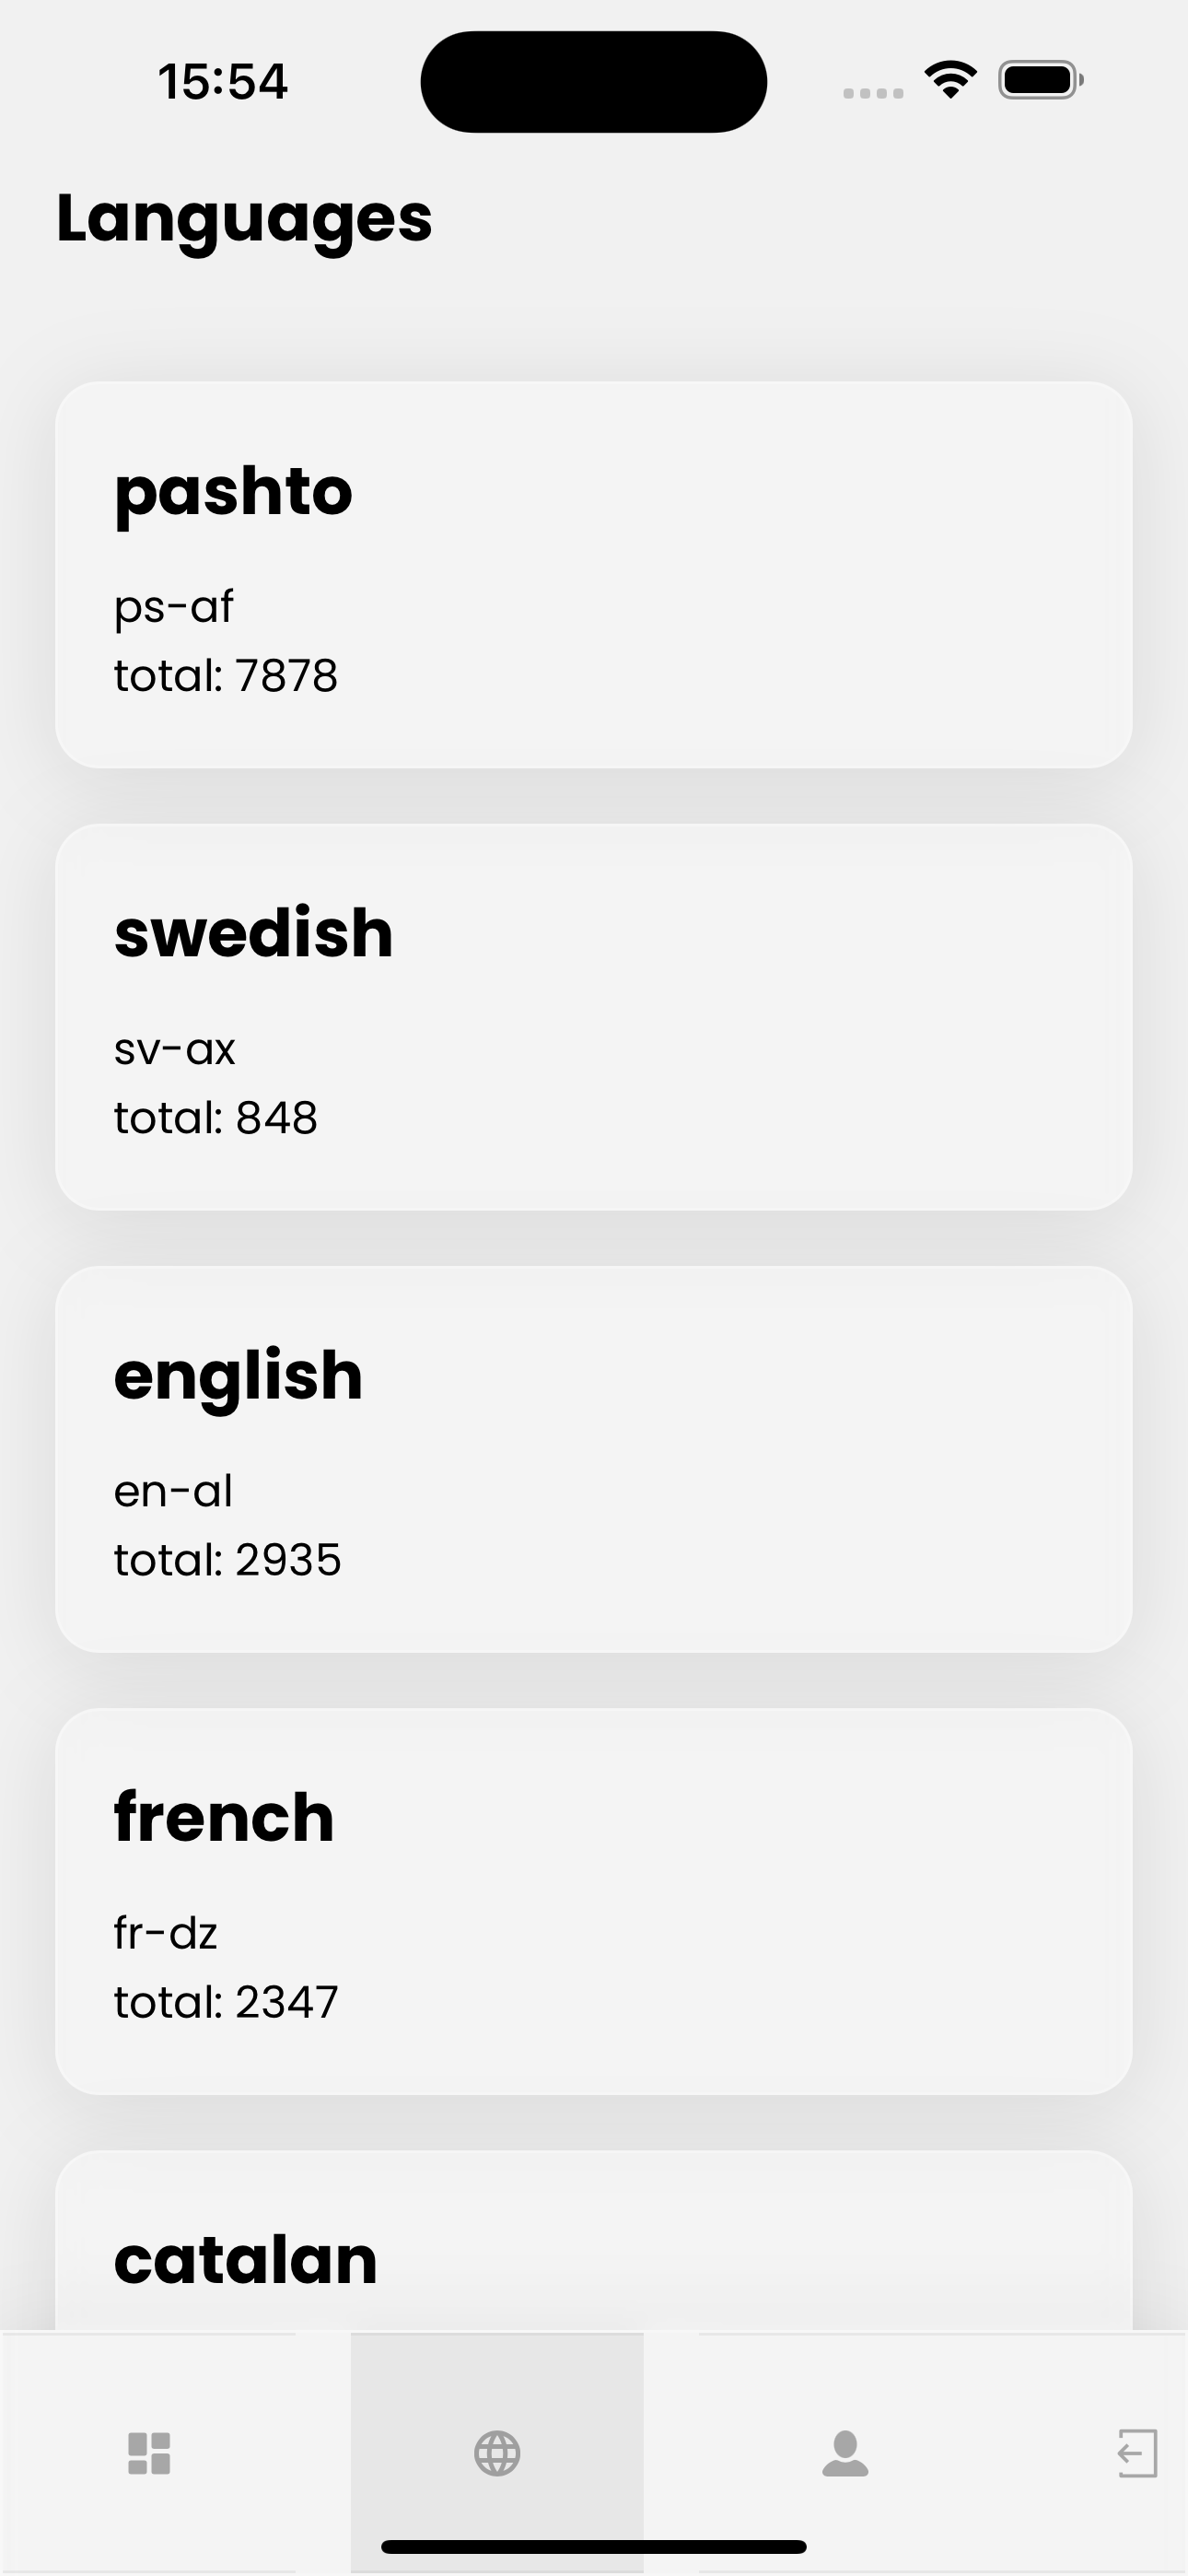
\includegraphics[width=0.4\textwidth]{assets/16.png}
  \end{figure}


  \begin{figure}
    \centering
    \caption{
     List of languages by movie inside iframe on the app.
    }
    \label{fig:app4}
    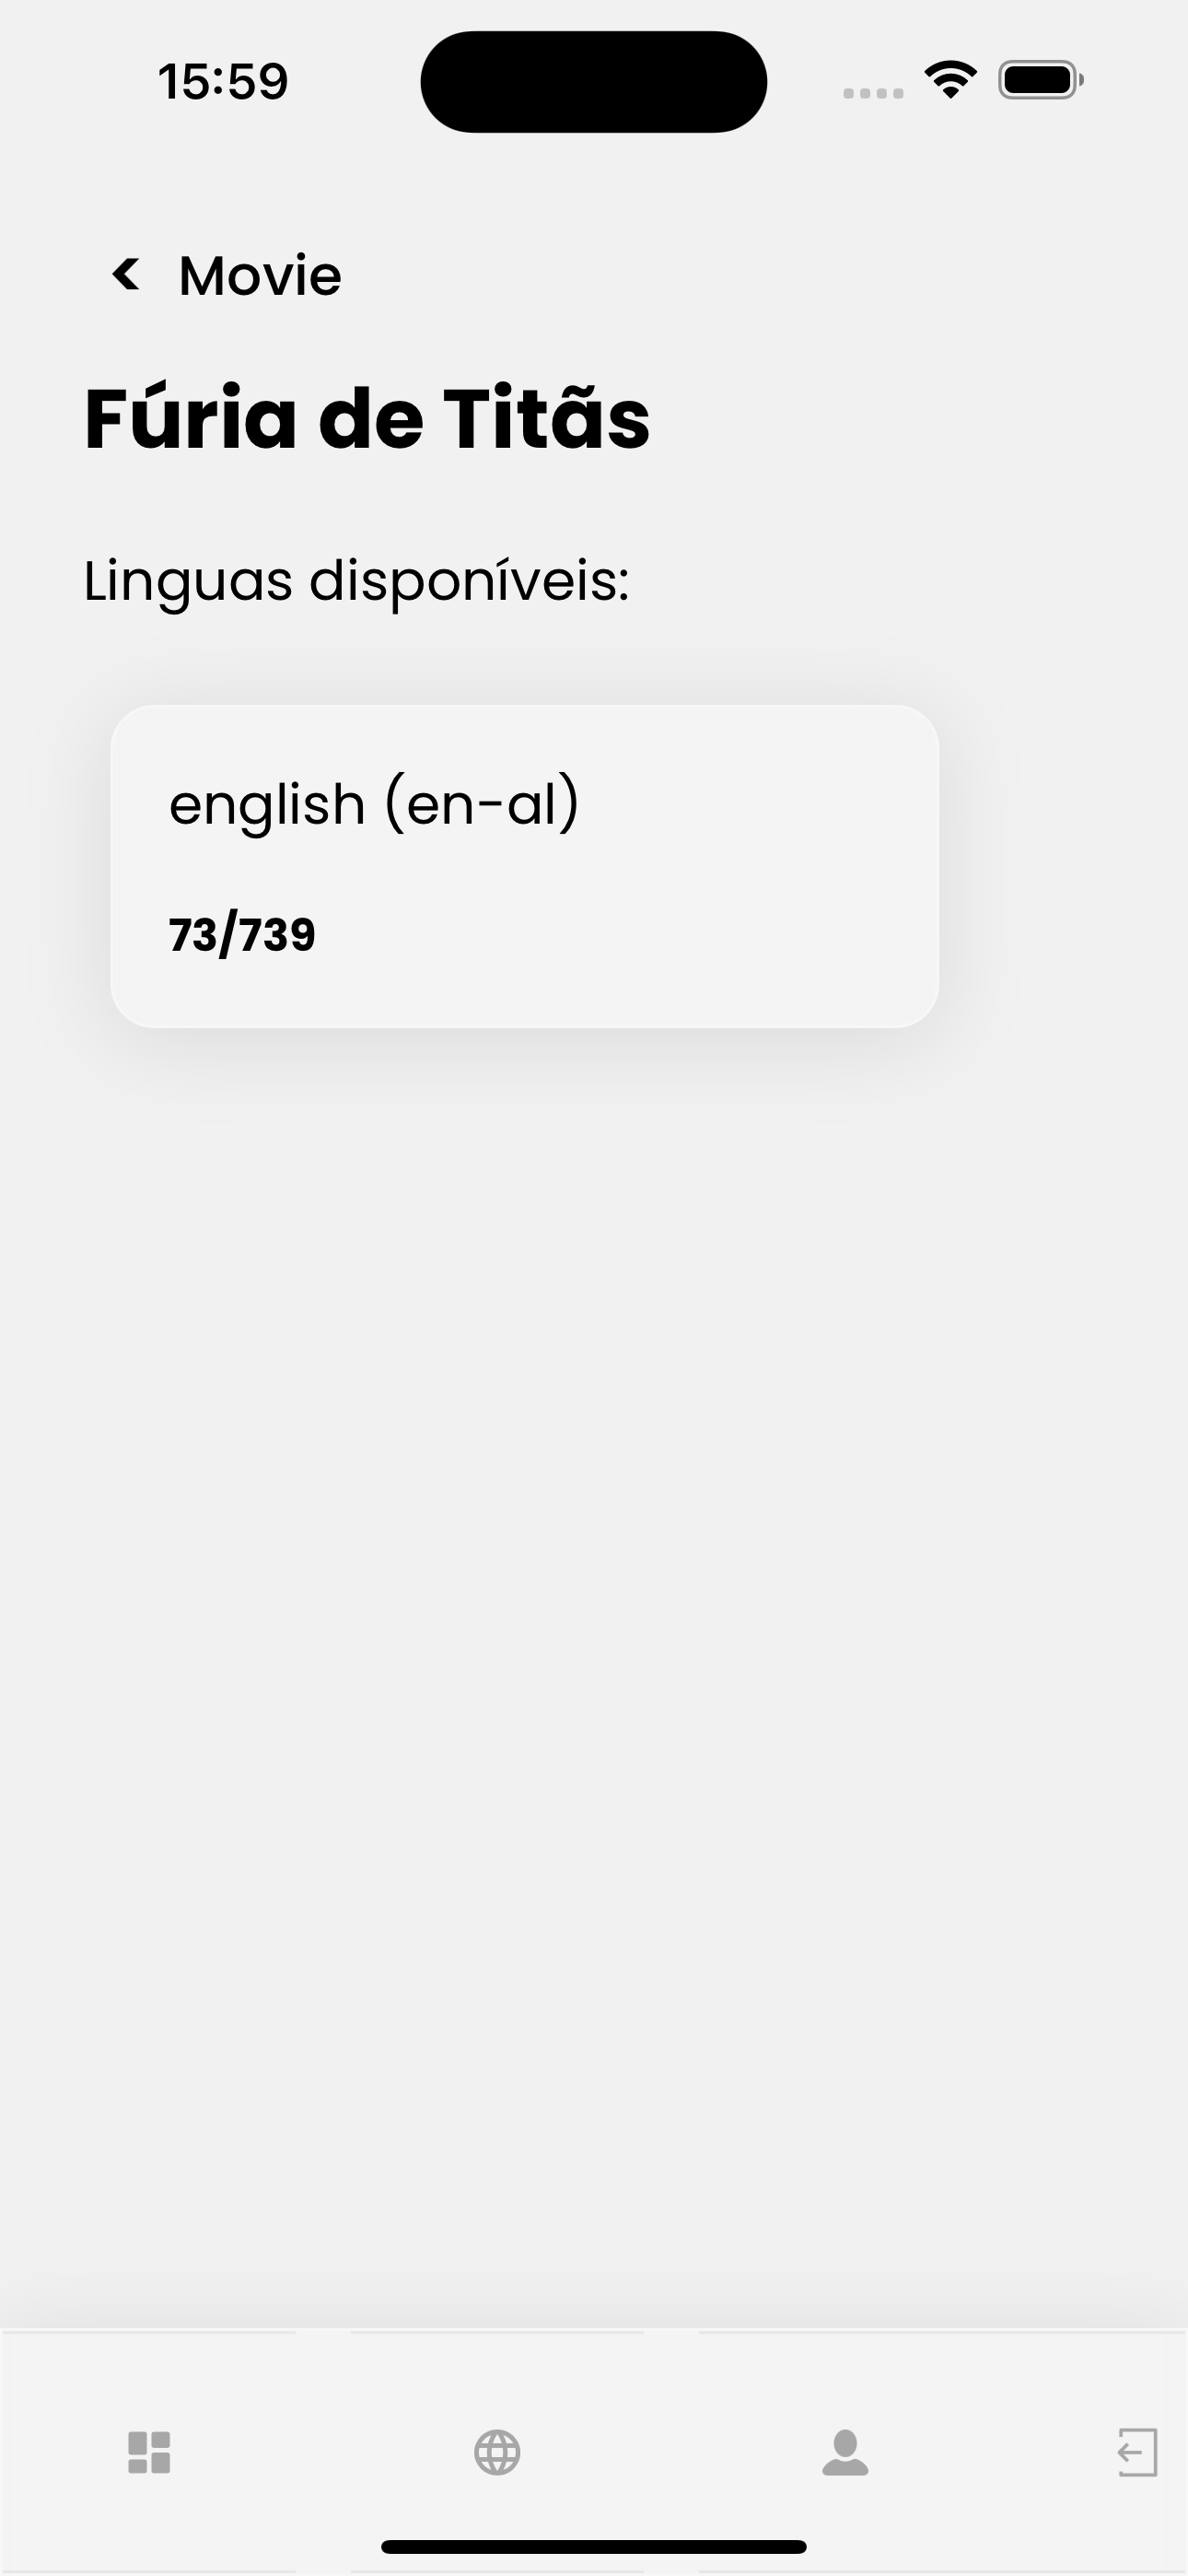
\includegraphics[width=0.4\textwidth]{assets/17.png}
  \end{figure}

  \begin{figure}
    \centering
    \caption{
     List of languages by movie inside iframe on the app.
    }
    \label{fig:app5}
    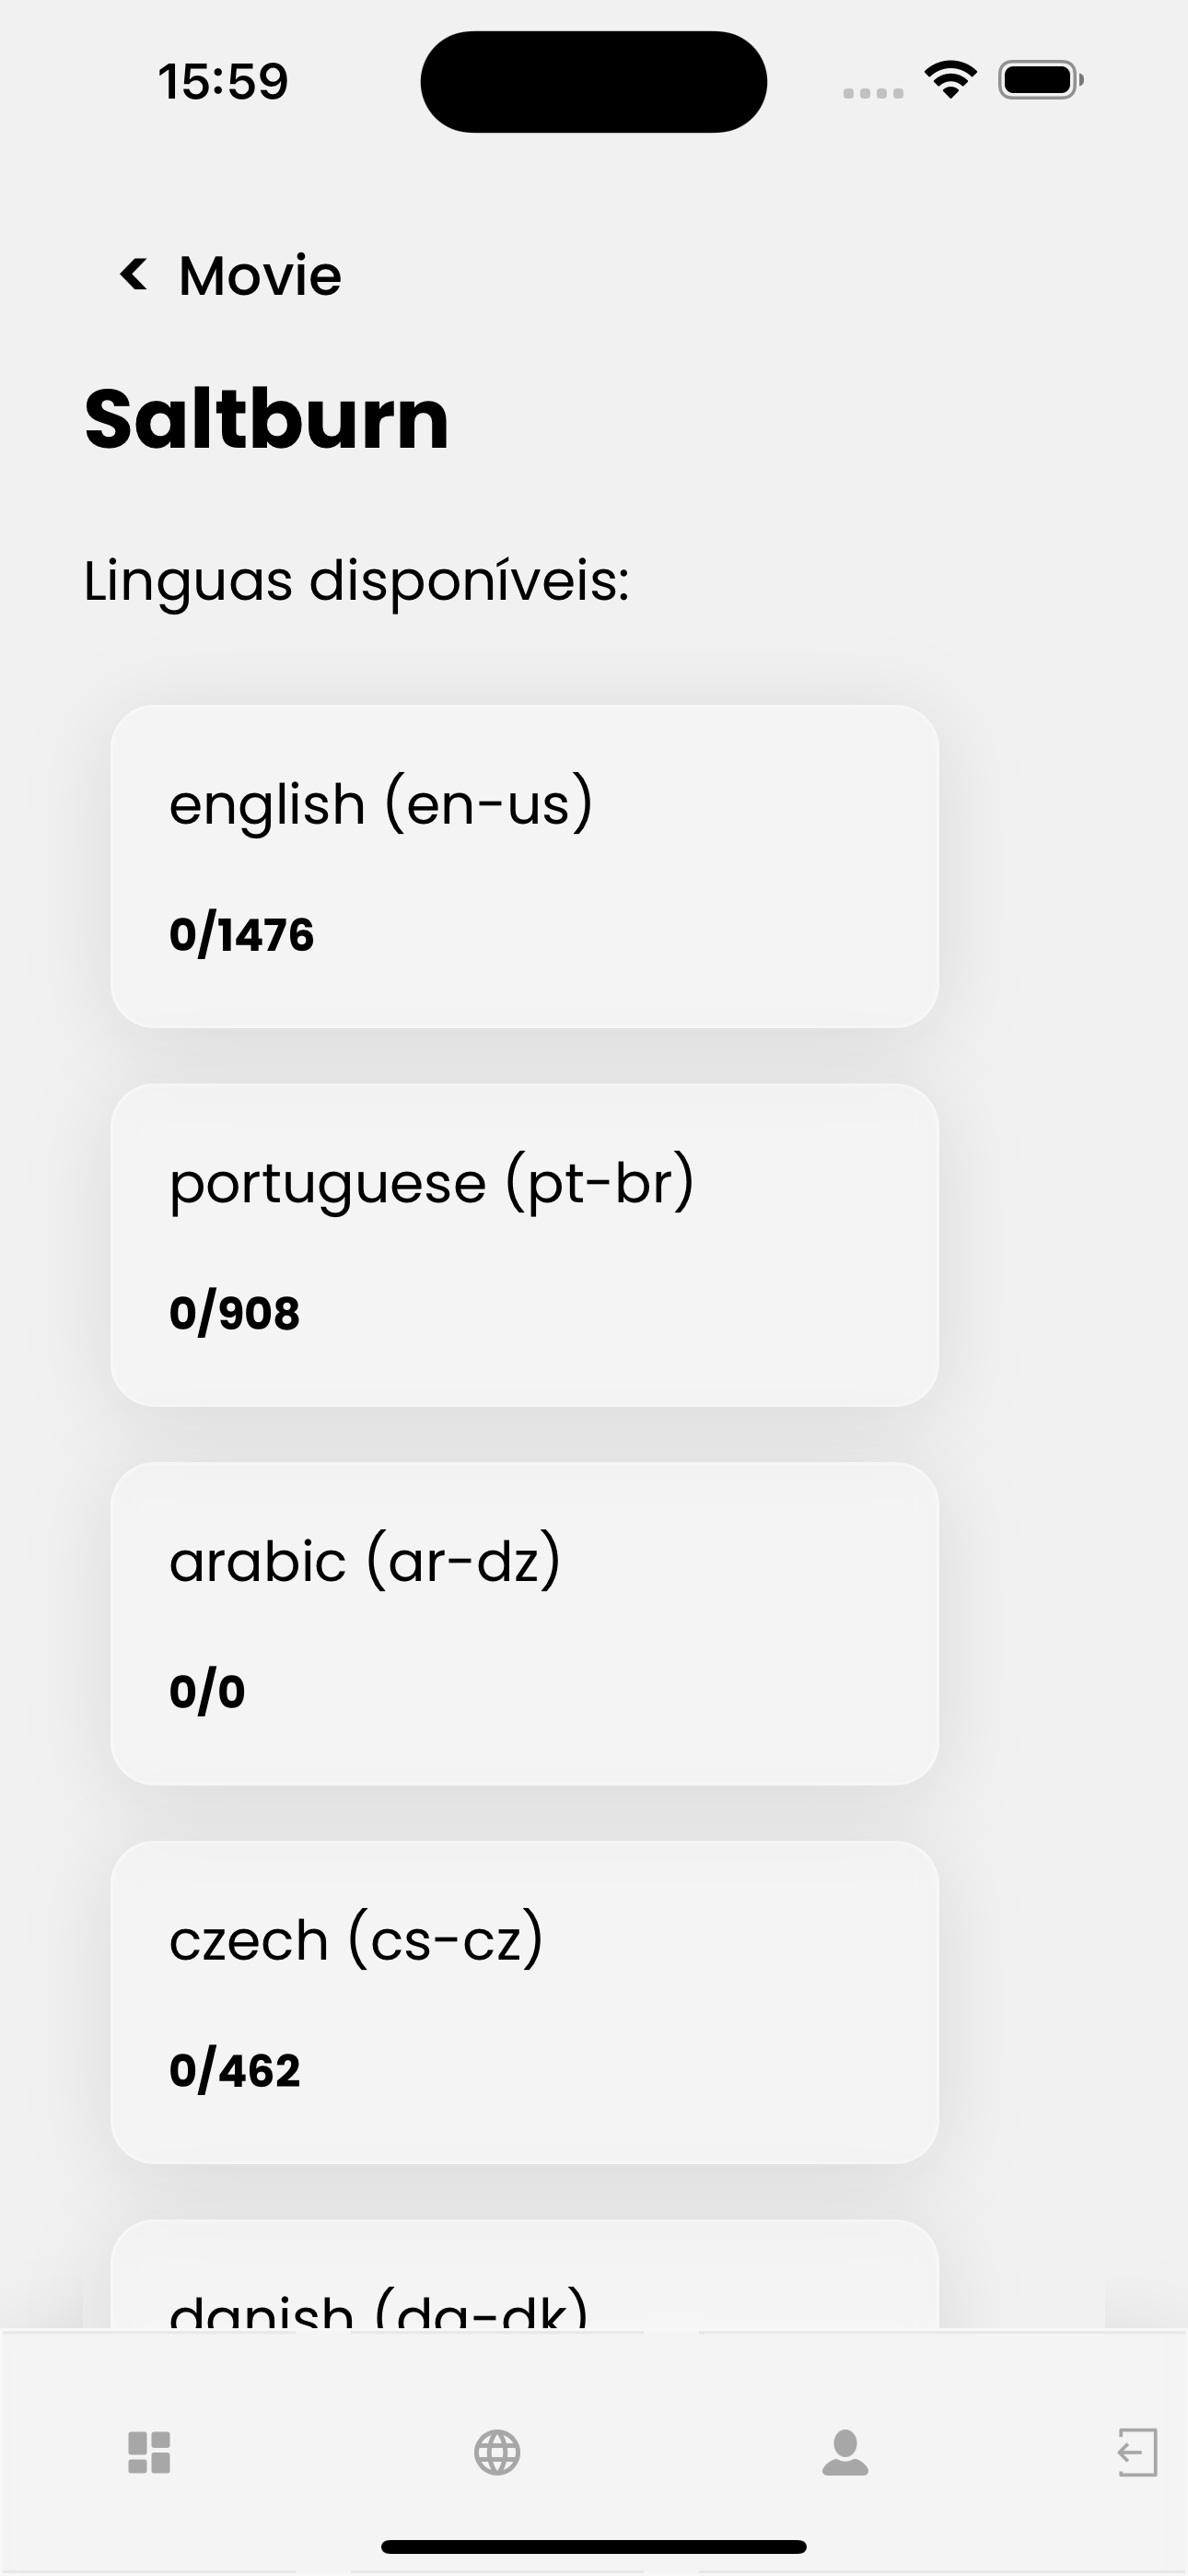
\includegraphics[width=0.4\textwidth]{assets/18.png}
  \end{figure}

  \begin{figure}
    \centering
    \caption{
     Translate game inside iframe on the app.
    }
    \label{fig:app6}
    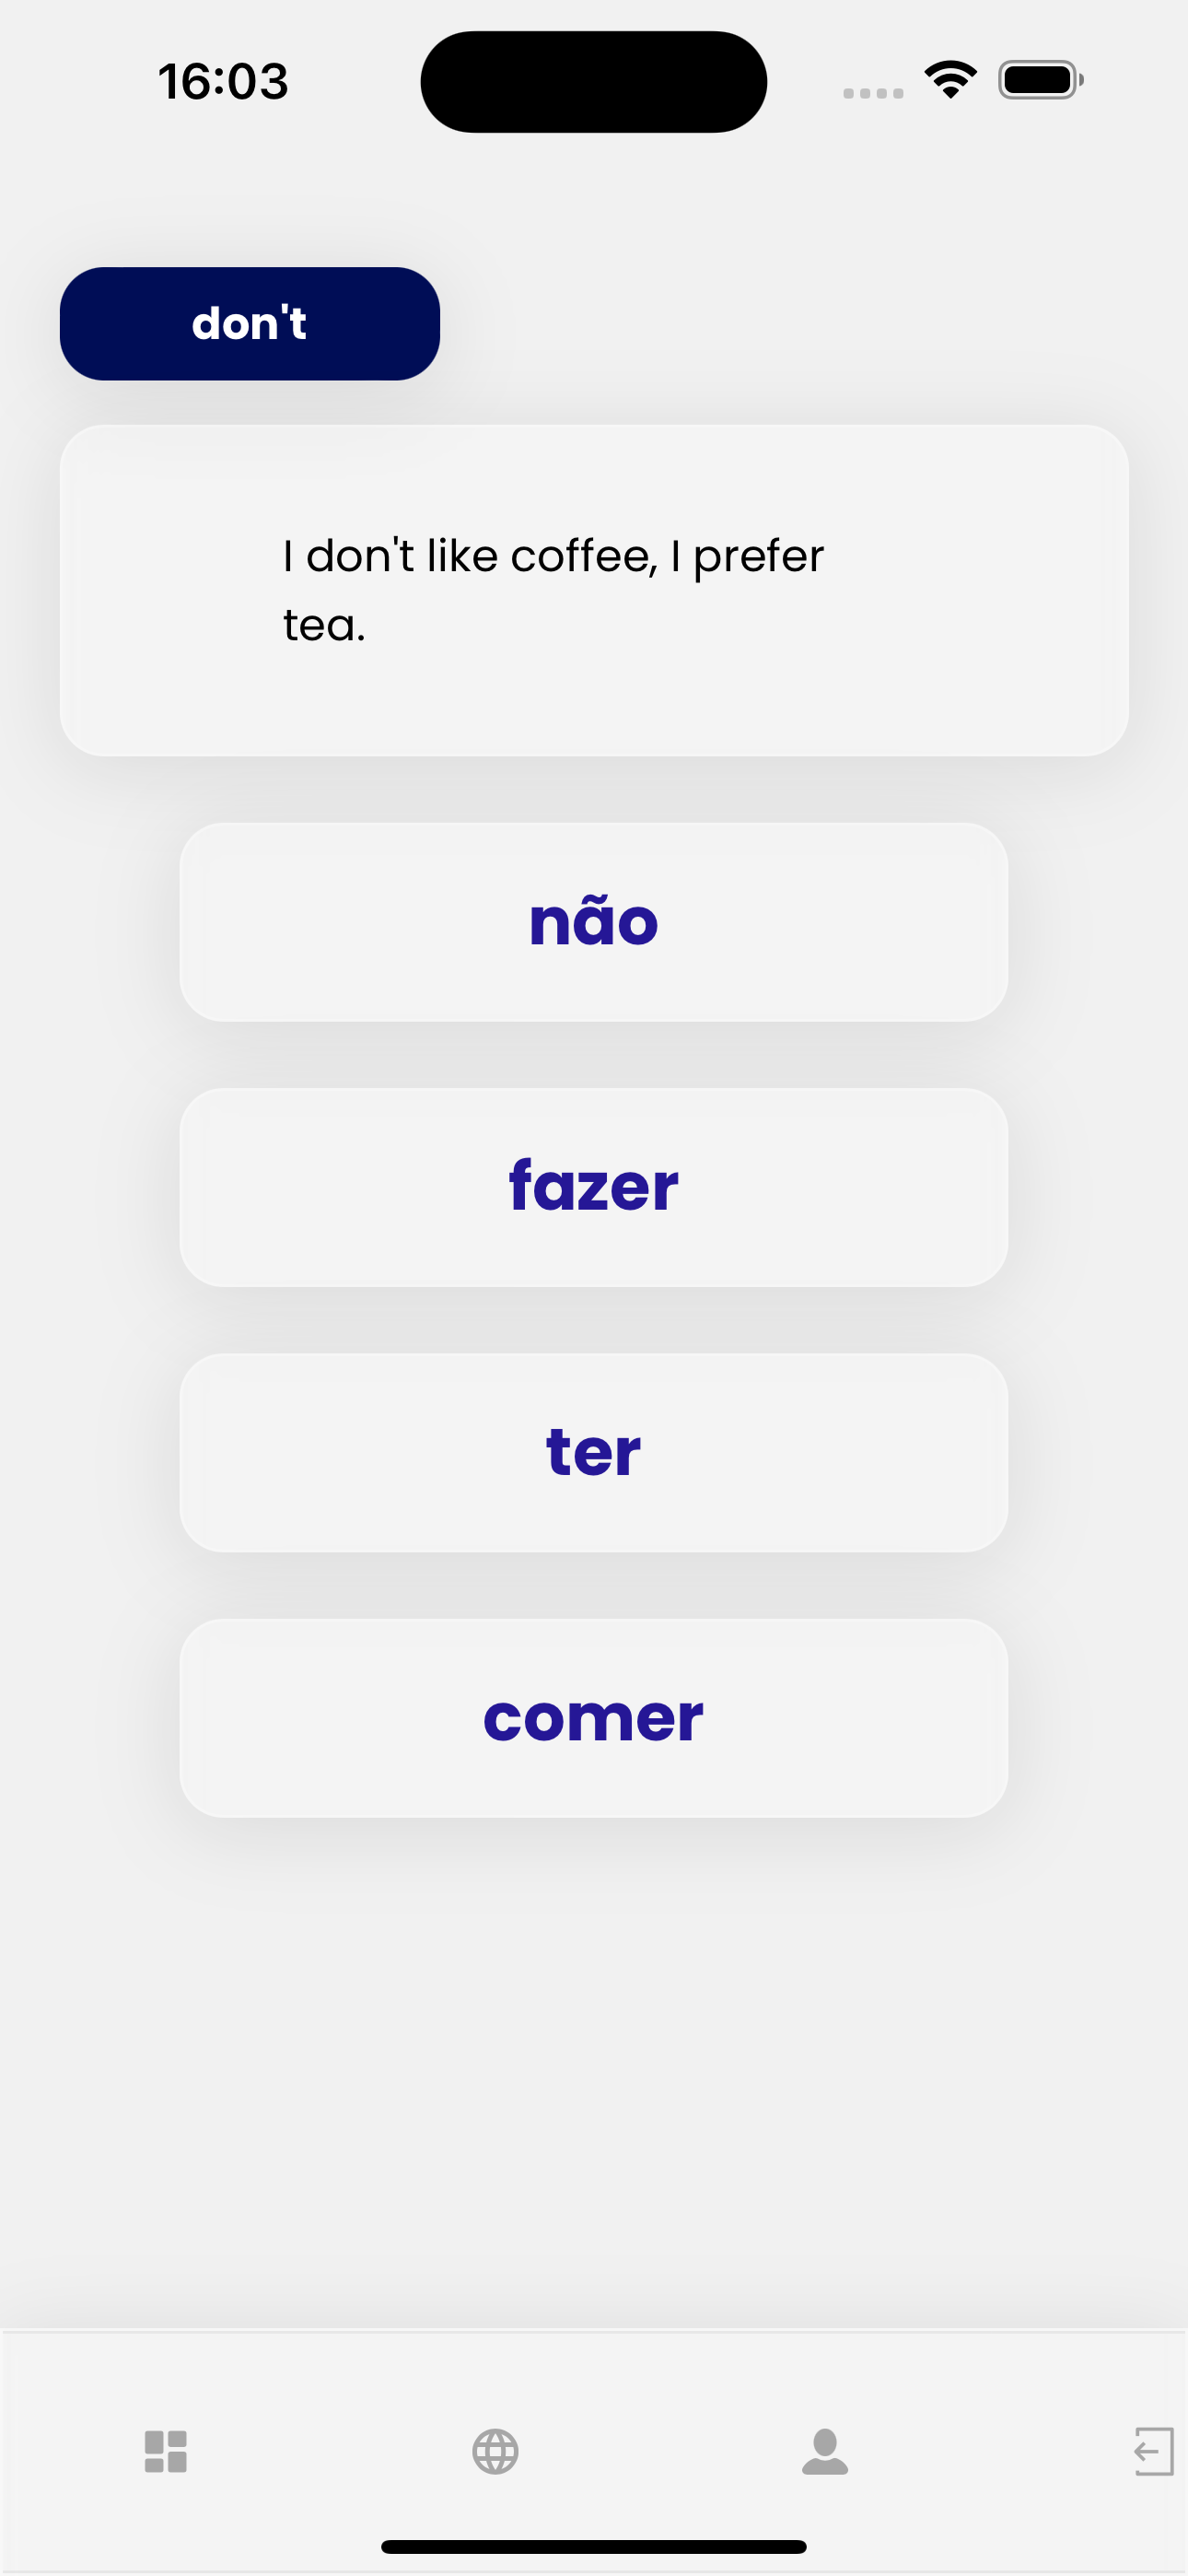
\includegraphics[width=0.4\textwidth]{assets/19.png}
  \end{figure}



\section{Next Steps}

For the next steps there are subsections for each one and each environment (extension, site, app).

\subsection{Extension}

List of next steps for the extension:

- Expanded to other streaming sites, languages, and platforms. 

- Use the browser's internal messaging services and, in the future, integrate with some web sockets to improve the communication between the extension and the site. 

- Integration with other language learning tools, such as Language Reactor, that uses a similar approach to the project but with a different focus. 

- New interactive exercises and games to reinforce vocabulary acquisition and customize the extension to the user's level and interests.

\subsection{Site}

List of next steps for the site:

- The site will be expanded to include new features like interactive exercises and games to reinforce vocabulary acquisition. The site will also be customized to the user's level and interests, providing an interactive and engaging learning environment. 

- New channels Will allow the site to communicate with mobile and notify the user to study like a reminder. 

- Web sockets will be used to improve the communication between the extension and the site.

- Redesign the site to improve the user experience and make it more responsive.

\subsection{App}

List of next steps for the App:

- The app will capture device information and send it to iframe to turn it more responsible and fast. 

- New channels will be created to communicate with the site and allow native features like notifications and others.

\subsection{Backend} 

List of next steps for the backend:

- Some API routers will be improved using workers because the data will be extensive, and the app and site will be faster and more responsive.

- The language manager will be changed using only the language name, not the language code. 

- Creating web sockets to improve the communication between the extension and the site.

\section{Conclusion}

In conclusion, this project has successfully developed a browser extension, a website, and an app that aims to facilitate language learning by extracting subtitles from movie streaming sites. The extension utilizes Spaced Repetition System (SRS) techniques to gamify language learning, while the website provides statistics on user progress and supports multiple languages. The app allows users to study on any device.

Moving forward, several next steps are planned for each project component. The extension will be expanded to other streaming sites, languages, and platforms and integrated with other language-learning tools. The website will include interactive exercises, games, and customized learning experiences. The app will capture device information and improve communication with the website.

In addition, the project's backend will be enhanced with improvements to API routers and the language manager. Web sockets will improve communication between the extension and the website.

Overall, this project demonstrates the potential of using technology to make language learning more engaging and accessible. By integrating language learning with everyday activities like watching movies, users can enhance their language skills in a fun and interactive way.

\bibliographystyle{sbc}
\bibliography{sbc-template}

\centering
\break

\begin{tabular}{@{}p{.5in}p{4in}@{}}
& \hrulefill \\
& \centerline{Guilherme A. Avelino} \\
\\ \\ \\ \\ 
\end{tabular}

\centering
\begin{tabular}{@{}p{.5in}p{4in}@{}}
& \hrulefill \\
& \centerline{J. Emanuel Cascone R. S.} \\
\\ \\
\end{tabular}

\end{document}